% Informe final del proyecto AgroReglas (INFO1148).
% Compilar desde documentacion/:  pdflatex Informe_AgroReglas.tex  (tres veces, para índice y referencias)
% Las tablas de datos se incluyen desde generado/, que produce `python3 generar_resultados.py`.
\documentclass[11pt,letterpaper]{article}
\usepackage[utf8]{inputenc}
\usepackage[T1]{fontenc}
\usepackage{lmodern}
\usepackage{textcomp}
\usepackage[provide=*,spanish]{babel}
\usepackage[margin=2.3cm,headheight=14pt]{geometry}
\usepackage{amsmath,amssymb}
\usepackage{color,colortbl}
\usepackage{graphicx}
\usepackage{array,longtable,tabularx,calc}
\usepackage{verbatim}
\usepackage{fancyhdr}
\usepackage{url}
\usepackage[colorlinks=true,linkcolor=enlace,urlcolor=enlace,citecolor=enlace,
            pdftitle={Diseño e implementación de un analizador sintáctico: AgroReglas},
            pdfauthor={Juan Claudio Cárdenas Uribe; Juan Esteban Llanca Hernández; Bayron Rodrigo Flores Riquelme}]{hyperref}

\definecolor{acento}{rgb}{0.11,0.36,0.20}
\definecolor{enlace}{rgb}{0.06,0.28,0.55}
\definecolor{gris}{gray}{0.38}
\definecolor{fondo}{gray}{0.94}
\definecolor{cabecera}{rgb}{0.88,0.93,0.88}

\DeclareUnicodeCharacter{03B5}{\ensuremath{\varepsilon}}
\DeclareUnicodeCharacter{2192}{\ensuremath{\rightarrow}}
\DeclareUnicodeCharacter{21D2}{\ensuremath{\Rightarrow}}
\DeclareUnicodeCharacter{2026}{...}
\DeclareUnicodeCharacter{251C}{+}
\DeclareUnicodeCharacter{2514}{\textasciigrave}
\DeclareUnicodeCharacter{2502}{|}
\DeclareUnicodeCharacter{2500}{-}
\DeclareUnicodeCharacter{2713}{\ensuremath{\checkmark}}
\DeclareUnicodeCharacter{2212}{-}
\DeclareUnicodeCharacter{03B2}{\ensuremath{\beta}}
\DeclareUnicodeCharacter{0663}{\textlangle U+0663\textrangle}

\setlength{\parindent}{0pt}
\setlength{\parskip}{5pt plus 1pt}
\setlength{\emergencystretch}{3em}
\renewcommand{\arraystretch}{1.18}
\setcounter{tocdepth}{2}
\setlength{\LTcapwidth}{\linewidth}

\makeatletter
\renewcommand\section{\@startsection{section}{1}{\z@}{-3.2ex \@plus -1ex \@minus -.2ex}{1.6ex \@plus .2ex}%
  {\normalfont\Large\bfseries\color{acento}}}
\renewcommand\subsection{\@startsection{subsection}{2}{\z@}{-2.6ex\@plus -1ex \@minus -.2ex}{1.0ex \@plus .2ex}%
  {\normalfont\large\bfseries}}
\renewcommand\subsubsection{\@startsection{subsubsection}{3}{\z@}{-2ex\@plus -1ex \@minus -.2ex}{0.6ex \@plus .2ex}%
  {\normalfont\normalsize\bfseries}}
\newcommand{\captionof}[1]{\def\@captype{#1}\caption}
\newcommand{\filas}[1]{\@@input #1 }
% Salta de página si queda menos espacio que #1 (como el paquete needspace).
\newcommand{\necesita}[1]{\par\penalty-100\begingroup\setlength{\dimen@}{#1}%
  \dimen@ii\pagegoal\advance\dimen@ii-\pagetotal
  \ifdim\dimen@>\dimen@ii\ifdim\dimen@ii>\z@\vfil\fi\break\fi\endgroup}
\makeatother
\AtBeginDocument{\renewcommand{\tablename}{Tabla}\renewcommand{\listtablename}{Índice de tablas}}

\pagestyle{fancy}
\fancyhf{}
\fancyhead[L]{\small\color{gris}INFO1148 --- Proyecto de análisis sintáctico}
\fancyhead[R]{\small\color{gris}AgroReglas}
\fancyfoot[C]{\small\thepage}
\renewcommand{\headrulewidth}{0.4pt}

\newcommand{\cod}[1]{\texttt{#1}}
\newcommand{\ruta}[1]{\nolinkurl{#1}}
\newcommand{\T}[1]{\texttt{#1}}
\newcommand{\NT}[1]{\textit{#1}}
\newcommand{\eps}{\ensuremath{\varepsilon}}
\newcommand{\flecha}{\ensuremath{\rightarrow}}
\newcommand{\cabeza}{\rowcolor{cabecera}}
\newenvironment{codigo}{\par\small\vspace{2pt}}{\par\vspace{2pt}}
\newcommand{\archivo}[1]{\begingroup\small\verbatiminput{#1}\endgroup}
\newcommand{\archivopeq}[1]{\begingroup\footnotesize\verbatiminput{#1}\endgroup}
\newcommand{\archivomin}[1]{\begingroup\scriptsize\verbatiminput{#1}\endgroup}

\newcommand{\NumCasos}{59}
\newcommand{\NumValidas}{16}
\newcommand{\NumInvalidas}{22}
\newcommand{\NumLimite}{21}
\newcommand{\NumCorrectos}{59}
\newcommand{\NumMetodos}{75}
\newcommand{\NumCeldas}{31}
\newcommand{\NumCeldasError}{179}
\newcommand{\NumConflictosGcero}{6}
\newcommand{\NumConflictosGuno}{9}
\newcommand{\PasosDerivacion}{19}
\newcommand{\PasosTraza}{26}
\newcommand{\PasadasFirst}{5}
\newcommand{\PasadasFollow}{3}
\newcommand{\NumEjemplos}{15}
\newcommand{\NumAleatoriasLexico}{3000}
\newcommand{\NumComparadasLexico}{3000}
\newcommand{\NumDiferenciales}{1200}
\newcommand{\NumDiferencialesAceptadas}{351}
\newcommand{\NumDiferencialesRechazadas}{849}
\newcommand{\NumEarleyAceptadas}{351}
\newcommand{\NumOracionesGcero}{300}
\newcommand{\NumMutacionesInmediata}{600}
\newcommand{\LineasExtractoParser}{agroreglas/parser.py, líneas 181--230}
\newcommand{\LineasExtractoFirstFollow}{agroreglas/ll1.py, líneas 35--79}
\newcommand{\LineasExtractoTabla}{agroreglas/ll1.py, líneas 82--108}
\newcommand{\LineasExtractoSemantica}{agroreglas/abstracto.py, líneas 84--108}
\newcommand{\LineasExtractoViables}{agroreglas/parser.py, líneas 122--133}
\newcommand{\EntradaDerivacion}{\texttt{WHEN \allowbreak{}humedad \allowbreak{}\textless{} \allowbreak{}30 \allowbreak{}AND \allowbreak{}NOT \allowbreak{}lluvia \allowbreak{}== \allowbreak{}TRUE \allowbreak{}THEN \allowbreak{}regar \allowbreak{}sector\_\allowbreak{}sur \allowbreak{}DURING \allowbreak{}15;}}
\newcommand{\EntradaTraza}{\texttt{WHEN \allowbreak{}h \allowbreak{}\textless{} \allowbreak{}1 \allowbreak{}THEN \allowbreak{}a \allowbreak{}b \allowbreak{}DURING \allowbreak{}2;}}


\begin{document}

% ------------------------------------------------------------------ portada
\begin{titlepage}
\centering
{\large Universidad Católica de Temuco\\[2pt] Ingeniería Civil Informática\par}
\vspace{0.6cm}
{\large Teoría de la Computación --- INFO1148\par}
\vspace{2.6cm}
{\color{acento}\rule{0.75\linewidth}{1pt}\par}
\vspace{0.5cm}
{\LARGE\bfseries Diseño e implementación de un analizador sintáctico:\\[6pt] AgroReglas\par}
\vspace{0.4cm}
{\large Un lenguaje de reglas para la automatización del riego agrícola\par}
\vspace{0.5cm}
{\color{acento}\rule{0.75\linewidth}{1pt}\par}
\vspace{0.8cm}
{\normalsize Gramática libre de contexto · FIRST y FOLLOW · Tabla LL(1)\\
Parser predictivo dirigido por tabla · Árbol concreto y AST · Errores localizados\par}
\vfill
\begin{tabular}{rl}
\textbf{Integrantes:} & Juan Claudio Cárdenas Uribe\\
 & Juan Esteban Llanca Hernández\\
 & Bayron Rodrigo Flores Riquelme\\[8pt]
\textbf{Docente:} & Prof. M. Lévano\\[8pt]
\textbf{Fecha:} & 14 de noviembre de 2026\\[8pt]
\textbf{Repositorio:} & \url{https://github.com/der-kaffe/AgroReglas-LL1}
\end{tabular}
\vfill
{\small\color{gris}Python 3.10 o superior · solo biblioteca estándar · sin generadores de parsers\par}
\end{titlepage}

\begingroup\setlength{\parskip}{1pt}\tableofcontents\endgroup
\clearpage

% ====================================================================== 1
\section{Introducción y dominio seleccionado}\label{sec:intro}

Los lenguajes de dominio específico (DSL) permiten que una persona experta en un área describa
comportamientos sin escribir un programa general. Para que una herramienta pueda procesar esas
descripciones, primero debe verificar que la secuencia de símbolos respeta una estructura formal. Este
proyecto diseña un DSL pequeño, lo formaliza con una gramática libre de contexto (GLC), la analiza y la
transforma hasta obtener una gramática LL(1), y construye a mano un analizador sintáctico predictivo que
acepta programas válidos, rechaza los inválidos con mensajes localizados y produce un árbol sintáctico
concreto y un árbol de sintaxis abstracta (AST).

\paragraph{Dominio.} Se eligió la automatización del riego agrícola, uno de los dominios sugeridos por el
enunciado. Un programa AgroReglas es una lista de reglas del tipo «cuando se cumpla esta condición sobre los
sensores del campo, solicitar estas acciones sobre los equipos»:

\begin{codigo}
\begin{verbatim}
WHEN humedad < 30 AND NOT (lluvia == TRUE OR viento > 40)
THEN regar sector_norte DURING 15 AND activar alarma;
\end{verbatim}
\end{codigo}

La regla pide regar el sector norte durante 15 minutos y activar una alarma cuando la humedad del suelo
es baja, siempre que no esté lloviendo ni haya viento fuerte. El dominio es adecuado porque las condiciones
combinan comparaciones con conectores lógicos, negación y agrupación ---lo que obliga a resolver
precedencia y ambigüedad en la gramática---, y porque la duración del riego da lugar a una construcción propia
del dominio: la cláusula opcional \T{DURING} \textit{minutos}.

\paragraph{Alcance.} El proyecto realiza \textbf{reconocimiento sintáctico}: decide si un texto pertenece al
lenguaje, informa el primer error y construye árboles. No ejecuta reglas, no evalúa condiciones, no valida
la semántica (por ejemplo, que \T{humedad} sea un sensor existente o que \T{regar} se aplique a un sector) y
no controla equipos reales. Esa separación se hace explícita en la sección~\ref{sec:restricciones} y en el
caso de prueba L21, que es sintácticamente válido aunque no tenga sentido en el dominio.

\paragraph{Resultados principales.} La gramática final tiene 14 no terminales, 14 terminales y
23 producciones; se obtuvo desde una versión inicial ambigua y recursiva por la izquierda (G0, con
\NumConflictosGcero{} conflictos LL(1)) pasando por una versión con niveles de precedencia (G1, con
\NumConflictosGuno{} conflictos) hasta la versión final G2, sin conflictos. FIRST, FOLLOW, los conjuntos de
selección y la tabla se calculan con algoritmos propios y coinciden con el cálculo manual. Se ejecutaron
\NumCasos{} entradas documentadas (\NumValidas{} válidas, \NumInvalidas{} inválidas y \NumLimite{} casos
límite), todas con el resultado esperado, y \NumMetodos{} métodos de prueba automatizados que, además, evalúan
miles de entradas aleatorias y comparan el parser con un reconocedor independiente.

\paragraph{Organización.} El informe sigue la estructura sugerida en el enunciado: especificación del
lenguaje (sección~\ref{sec:especificacion}), gramática (\ref{sec:glc}), análisis (\ref{sec:analisis}),
FIRST y FOLLOW (\ref{sec:firstfollow}), tabla LL(1) (\ref{sec:tabla}), parser (\ref{sec:parser}),
árboles (\ref{sec:arboles}), errores (\ref{sec:errores}), pruebas (\ref{sec:pruebas}), conclusiones
(\ref{sec:conclusiones}) y anexos (\ref{sec:anexos}), que incluyen el repositorio, las evidencias de ejecución
y la trazabilidad con la rúbrica.

% ====================================================================== 2
\section{Especificación del lenguaje}\label{sec:especificacion}

\subsection{Propósito}
AgroReglas describe reglas de automatización de riego. Cada regla tiene una \emph{condición} sobre lecturas
de sensores (humedad, lluvia, viento, temperatura, nivel de un tanque, radiación, etc.) y una o más
\emph{acciones}, cada una formada por un verbo y un objetivo (\T{regar sector\_norte},
\T{abrir valvula\_1}) y, opcionalmente, una duración en minutos. Un programa contiene una o más reglas
independientes, cada una terminada en punto y coma.

\subsection{Alfabeto}
El alfabeto relevante $\Sigma$ está formado por:
\begin{itemize}
\item letras ASCII \T{A}--\T{Z} y \T{a}--\T{z}, dígitos ASCII \T{0}--\T{9} y el guion bajo \T{\_};
\item los caracteres de operadores \T{<}, \T{>}, \T{=} y \T{!} (los dos últimos solo dentro de \T{==}, \T{!=},
      \T{<=} y \T{>=});
\item los separadores \T{;}, \T{(} y \T{)};
\item los blancos espacio, tabulación (\T{\textbackslash t}), retorno de carro (\T{\textbackslash r}) y salto
      de línea (\T{\textbackslash n}), que separan tokens y se descartan.
\end{itemize}
Cualquier otro carácter (por ejemplo \T{@}, \T{,}, \T{.}, \T{-}, \T{ñ}, letras con tilde o dígitos no ASCII)
produce un error léxico con su ubicación.

\subsection{Categorías de tokens y patrones}
El analizador léxico usa expresiones regulares combinadas en un único patrón, en el mismo orden que el
notebook docente (la primera alternativa que coincide gana y cada operador de dos caracteres aparece antes que
su prefijo de uno). La tabla~\ref{tab:tokens} resume las categorías.

\begin{longtable}{>{\raggedright}p{2.9cm}>{\raggedright}p{4.4cm}>{\raggedright}p{3.6cm}p{4.3cm}}
\caption{Categorías de tokens de AgroReglas.}\label{tab:tokens}\\
\hline\cabeza \textbf{Token} & \textbf{Patrón} & \textbf{Ejemplos} & \textbf{Uso}\\\hline\endfirsthead
\hline\cabeza \textbf{Token} & \textbf{Patrón} & \textbf{Ejemplos} & \textbf{Uso}\\\hline\endhead
\T{WHEN}, \T{THEN} & palabra reservada & \T{WHEN}, \T{then} & inicio de regla; separa condición y acciones\\
\T{AND}, \T{OR}, \T{NOT} & palabra reservada & \T{AND}, \T{not} & conectores lógicos; \T{AND} también separa acciones\\
\T{TRUE}, \T{FALSE} & palabra reservada & \T{TRUE}, \T{false} & valores booleanos\\
\T{DURING} & palabra reservada & \T{DURING}, \T{during} & extensión: duración de una acción\\
\T{ID} & \T{[A-Za-z\_][A-Za-z0-9\_]*} & \T{humedad}, \T{valvula\_1}, \T{\_h} & sensores, verbos y objetivos\\
\T{NUM} & \T{[0-9]+} & \T{0}, \T{30}, \T{007} & enteros sin signo, sin límite de dígitos\\
\T{OP\_REL} & \T{>= | <= | == | != | > | <} & \T{<}, \T{>=}, \T{!=} & operadores relacionales\\
\T{PUNTO\_COMA} & \T{;} & \T{;} & fin de regla\\
\T{PARENT\_IZQ} & \T{\textbackslash(} & \T{(} & abre agrupación\\
\T{PARENT\_DER} & \T{\textbackslash)} & \T{)} & cierra agrupación\\
(ESPACIO) & \T{[ \textbackslash t\textbackslash r\textbackslash n]+} & espacio, salto & se descarta\\
(ERROR) & \T{.} (cualquier otro) & \T{@}, \T{,}, \T{=} & error léxico\\
\T{EOF} & --- (sintético) & --- & fin de entrada, agregado por el lexer\\\hline
\end{longtable}

\subsection{Palabras reservadas, identificadores, valores, operadores y separadores}
\begin{itemize}
\item \textbf{Palabras reservadas (8):} \T{WHEN}, \T{THEN}, \T{AND}, \T{OR}, \T{NOT}, \T{TRUE}, \T{FALSE} (las
siete del notebook docente) y \T{DURING} (extensión). Un lexema con forma de identificador cuyo texto en
mayúsculas coincide con una reservada se convierte en ese token; por eso una reservada no puede usarse como
identificador (caso I22).
\item \textbf{Identificadores:} nombran sensores (a la izquierda de una comparación), verbos (primer
identificador de una acción) y objetivos (segundo identificador). El rol depende de la posición en la
gramática, no del texto: el lenguaje no tiene un catálogo cerrado de sensores ni de acciones.
\item \textbf{Valores:} números enteros sin signo (\T{NUM}; \T{007} vale 7) y booleanos \T{TRUE}/\T{FALSE}. Un
valor solo puede aparecer a la derecha de un operador relacional o después de \T{DURING} (solo \T{NUM}).
\item \textbf{Operadores:} seis relacionales (\T{<}, \T{<=}, \T{>}, \T{>=}, \T{==}, \T{!=}, todos de la categoría
\T{OP\_REL}) y tres lógicos (\T{NOT}, \T{AND}, \T{OR}), con precedencia \T{NOT} $>$ \T{AND} $>$ \T{OR}.
\item \textbf{Separadores:} \T{;} termina cada regla; \T{(} y \T{)} agrupan condiciones; \T{THEN} separa la
condición de las acciones; dentro de las acciones, \T{AND} separa una acción de la siguiente.
\end{itemize}

\subsection{Mayúsculas, blancos y fin de entrada}
\begin{itemize}
\item Las palabras reservadas no distinguen mayúsculas (\T{when}, \T{When} y \T{WHEN} son el mismo token),
igual que en la función docente; el lexema original se conserva. Los identificadores sí las distinguen:
\T{Humedad} y \T{humedad} son identificadores distintos.
\item Los blancos se descartan. Solo son necesarios entre dos palabras (\T{WHENh} es un único identificador);
alrededor de operadores y paréntesis son opcionales (\T{WHEN(humedad<30)THEN ...}, caso L07). Se acepta el
fin de línea CRLF.
\item Al terminar el texto, el lexer agrega el token sintético \T{EOF}, que corresponde al marcador \$ del
análisis LL(1). La consola tolera además la marca BOM de UTF-8 que agregan algunos editores.
\end{itemize}

\subsection{Restricciones y casos excluidos}\label{sec:restricciones}
Quedan fuera del lenguaje, y se rechazan: programas vacíos o formados solo por blancos; reglas sin condición o
sin acciones; sentencias vacías (\T{;;}); números decimales o con signo; comas; comentarios; cadenas de texto;
identificadores o números a ambos lados de una comparación (el lado izquierdo es siempre un \T{ID} y el derecho un
\T{NUM} o un booleano); expresiones aritméticas; un booleano aislado como condición; \T{DURING} sin minutos, con
un booleano, repetido o fuera de una acción; letras no ASCII en los identificadores.

Por otra parte, hay entradas \emph{sintácticamente válidas} que una fase semántica posterior debería
rechazar: \T{DURING 0}, comparar booleanos con operadores de orden (\T{lluvia > TRUE}), usar un sensor como
objetivo o un verbo inexistente (caso L21). El analizador las acepta porque cumplen la gramática; validarlas
exigiría tipos, unidades, rangos y catálogos de equipos, que no forman parte de este proyecto.

\subsection{Cumplimiento de los requisitos mínimos}
\begin{longtable}{>{\raggedright}p{5.2cm}p{10.6cm}}
\caption{Requisitos mínimos del enunciado y cómo se cumplen.}\\
\hline\cabeza \textbf{Requisito} & \textbf{Cumplimiento en AgroReglas}\\\hline\endfirsthead
Al menos 4 palabras reservadas & 8: \T{WHEN THEN AND OR NOT TRUE FALSE DURING}\\
Identificadores & \T{ID}: sensores, verbos y objetivos\\
Valores numéricos y/o booleanos & \T{NUM} (enteros) y \T{TRUE}/\T{FALSE}\\
Al menos 3 operadores & 9: seis relacionales y tres lógicos\\
Estructura de sentencia principal & \T{WHEN} \textit{condición} \T{THEN} \textit{acciones} \T{;}\\
Más de una sentencia o regla & un programa es una secuencia de una o más reglas (\NT{Programa}, \NT{Resto})\\
Construcción compuesta & \T{AND}/\T{OR}, \T{NOT}, paréntesis y listas de acciones\\
Extensión creativa & \T{DURING} \textit{minutos} (propia del dominio), además de \T{NOT}, agrupación y varias acciones
(sección~\ref{sec:during})\\\hline
\end{longtable}

\subsection{Ejemplos válidos e inválidos}\label{sec:ejemplos}
Todos los ejemplos forman parte de la batería de pruebas (sección~\ref{sec:pruebas}); el identificador entre
corchetes remite a la tabla de resultados.

\textbf{Válidos.}
\begin{enumerate}
\item \T{WHEN humedad < 30 THEN regar sector\_norte;} [V01] --- la regla más simple: una comparación y una acción
con verbo y objetivo.
\item \T{WHEN lluvia != FALSE THEN activar alarma;} [V04] --- comparación con un valor booleano.
\item \T{WHEN (humedad < 20 OR temperatura > 35) AND lluvia == FALSE}\\ \T{THEN regar sector\_sur;} [V08] --- los
paréntesis hacen que el \T{OR} se agrupe antes que el \T{AND}.
\item \T{WHEN humedad < 30 THEN regar sector\_sur DURING 10 AND activar bomba;} [V10] --- dos acciones; solo la
primera indica duración.
\item \T{WHEN humedad < 25 THEN regar invernadero DURING 20;}\\
\T{WHEN viento > 60 THEN cerrar compuertas;} [V11] --- dos reglas en líneas distintas.
\item \T{when Lluvia == true then cerrar Valvula during 2;} [V13] --- reservadas en minúsculas; los
identificadores conservan su escritura.
\end{enumerate}

\textbf{Inválidos} (el mensaje real de cada uno aparece en la sección~\ref{sec:pruebas}).
\begin{enumerate}
\item \T{WHEN humedad < 30 regar sector\_sur;} [I01] --- falta \T{THEN}: tras la comparación solo pueden venir
\T{THEN}, \T{AND} u \T{OR}; el error se señala en \T{regar} (línea 1, columna 19).
\item \T{WHEN humedad < THEN regar sector\_sur;} [I02] --- falta el valor después del operador \T{<}.
\item \T{WHEN (humedad < 30 THEN regar sector\_sur;} [I06] --- el paréntesis abierto en la columna 6 no se cierra
antes de \T{THEN}.
\item \T{WHEN humedad < 30 THEN regar sector\_sur DURING TRUE;} [I10] --- \T{DURING} exige un número entero de
minutos.
\item \T{WHEN humedad < 30 THEN regar sector\_sur} [I04] --- falta el \T{;} final: la entrada termina con la regla
incompleta.
\item \T{WHEN humedad = 30 THEN regar sector\_sur;} [I19] --- \T{=} aislado no es un operador: error
\emph{léxico} con la sugerencia «¿Quiso escribir \T{==}?».
\end{enumerate}

\subsection{Componente léxico: base docente y modificaciones}\label{sec:lexico}
El enunciado permite usar la función entregada por el docente. El archivo original
\ruta{anlizador_lexico1.ipynb} se conserva intacto en \ruta{documentacion/} (una prueba verifica su
suma MD5) y \ruta{agroreglas/lexico.py} reproduce su función con las modificaciones de la
tabla~\ref{tab:modificaciones}.

\begin{longtable}{p{0.8cm}>{\raggedright}p{6.4cm}p{8.4cm}}
\caption{Modificaciones respecto del lexer del notebook docente.}\label{tab:modificaciones}\\
\hline\cabeza \textbf{Id} & \textbf{Cambio} & \textbf{Motivo}\\\hline\endfirsthead
\hline\cabeza \textbf{Id} & \textbf{Cambio} & \textbf{Motivo}\\\hline\endhead
M1 & \T{DURING} se agrega a las reservadas & extensión del dominio\\
M2 & cada token registra línea, columna (desde 1) y posición (desde 0) & mensajes de error localizados\\
M3 & se agrega el token final \T{EOF} & marcador \$ del análisis LL(1); detecta contenido sobrante y entradas truncadas\\
M4 & \T{ESPACIO} acepta \T{\textbackslash r} & archivos con fin de línea CRLF (Windows); el original los rechaza\\
M5 & \T{NUM} usa \T{[0-9]+} en vez de \T{\textbackslash d+} & en Python \T{\textbackslash d} acepta dígitos Unicode como U+0663 (tres arábigo-índico); así el
alfabeto queda en ASCII\\
M6 & error léxico \T{ErrorLexico} (subclase de \T{ValueError}) con ubicación y sugerencia & mismo tipo de excepción
que el original, con mensajes más útiles\\
M7 & \T{analizador\_lexico(cadena)} conserva la interfaz \T{[(TIPO, lexema), ...]} & comparar directamente con el
notebook y permitir que el parser reciba esos pares\\\hline
\end{longtable}

Se mantienen sin cambios las categorías, el orden de las alternativas, los patrones de \T{OP\_REL},
\T{PUNTO\_COMA}, paréntesis e \T{ID}, el descarte de blancos y la conversión de reservadas con \T{upper()}.

\textbf{Compatibilidad verificada.} En el \emph{subconjunto compartido} (texto ASCII, sin \T{\textbackslash r} y
sin la palabra \T{DURING}) ambas funciones deben producir la misma lista de pares o lanzar ambas
\T{ValueError}. Se comprobó con: (1) la salida que el docente dejó guardada en la segunda celda del notebook;
(2) las 42 entradas documentadas que pertenecen al subconjunto; y (3) \NumComparadasLexico{} cadenas
aleatorias construidas con fragmentos del alfabeto, incluidos símbolos inválidos. No hubo diferencias. Las
tres diferencias intencionales (M1, M4 y M5) se verifican por separado.

% ====================================================================== 3
\section{Gramática libre de contexto}\label{sec:glc}

\subsection{Definición formal}
La gramática final es $G_2 = (N, T, P, S)$, definida en \ruta{agroreglas/gramatica.py}; ese texto es la única
fuente de la gramática para el análisis, el parser, las tablas de este informe y los archivos de
\ruta{resultados/}.

\begin{itemize}
\item $N$ (14 no terminales): \NT{Programa}, \NT{Resto}, \NT{Regla}, \NT{Condicion}, \NT{ColaOr},
\NT{Conjuncion}, \NT{ColaAnd}, \NT{Factor}, \NT{Comparacion}, \NT{Valor}, \NT{Acciones}, \NT{ColaAcciones},
\NT{Accion}, \NT{Duracion}.
\item $T$ (14 terminales, que son categorías de token): \T{WHEN}, \T{THEN}, \T{ID}, \T{OP\_REL}, \T{NUM},
\T{TRUE}, \T{FALSE}, \T{NOT}, \T{AND}, \T{OR}, \T{PARENT\_IZQ}, \T{PARENT\_DER}, \T{DURING}, \T{PUNTO\_COMA}.
\item $S$ = \NT{Programa}.
\item $P$: las 23 producciones numeradas de la tabla~\ref{tab:producciones}. Los números se usan en la tabla
LL(1), en la traza del parser y en el código (reglas semánticas del AST).
\end{itemize}

\begin{longtable}{r>{\raggedright\arraybackslash}p{13.8cm}}
\caption{Producciones de $G_2$ (generado desde \cod{gramatica.py}).}\label{tab:producciones}\\
\hline\cabeza \textbf{N.º} & \textbf{Producción}\\\hline\endfirsthead
\hline\cabeza \textbf{N.º} & \textbf{Producción}\\\hline\endhead
\filas{generado/producciones.tex}
\hline
\end{longtable}

\subsection{Convenciones}
\begin{itemize}
\item $\varepsilon$ denota la cadena vacía: una producción $A \to \varepsilon$ permite que $A$ no genere nada.
En el código se representa con una tupla vacía.
\item \T{EOF} (equivalente a \$) \emph{no} pertenece a $T$: es un marcador de fin que se agrega al final de la
entrada. Se incorpora al análisis con $\mathrm{EOF} \in \mathrm{FOLLOW}(S)$ y como fondo de la pila del parser,
lo que equivale a aumentar la gramática con $S' \to S\ \mathrm{EOF}$.
\item Los terminales son categorías de token: \T{OP\_REL} representa a los seis operadores e \T{ID} a todos
los identificadores. Así, $L(G_2)$ es un lenguaje sobre categorías; el texto concreto se obtiene
reemplazando cada categoría por uno de sus lexemas.
\item Los no terminales se escriben en cursiva en el texto y sin tildes en el código (\NT{Condicion},
\NT{Accion}) para usar exactamente los mismos nombres en ambos.
\end{itemize}

\subsection{Lectura de la gramática}
\begin{itemize}
\item \textbf{Programa (1--3).} Una regla seguida de \NT{Resto}, que es otra regla y otro \NT{Resto}, o vacío: una
o más reglas.
\item \textbf{Regla (4).} \T{WHEN} \NT{Condicion} \T{THEN} \NT{Acciones} \T{;}.
\item \textbf{Condiciones (5--13).} Tres niveles fijan la precedencia: \NT{Condicion} une \NT{Conjuncion}es con
\T{OR} (menor precedencia); \NT{Conjuncion} une \NT{Factor}es con \T{AND}; \NT{Factor} es una negación, una
condición entre paréntesis o una comparación (mayor precedencia). \NT{ColaOr} y \NT{ColaAnd} representan
las repeticiones de cada conector.
\item \textbf{Comparación y valor (14--17).} Un sensor, un operador relacional y un número o booleano.
\item \textbf{Acciones (18--23).} Una acción seguida de \NT{ColaAcciones} (otras acciones precedidas de \T{AND}).
Cada acción es verbo, objetivo y una \NT{Duracion} opcional: \T{DURING} \T{NUM} o vacío.
\end{itemize}

\subsection{Derivación por la izquierda de una entrada válida}\label{sec:derivacion}
La tabla~\ref{tab:derivacion} muestra la derivación completa por la izquierda de
\EntradaDerivacion{}, que usa \T{AND}, \T{NOT} y la extensión \T{DURING}. En cada paso se reemplaza el no
terminal situado más a la izquierda; los terminales se muestran como categorías. La tabla se genera
recorriendo en preorden el árbol que construye el parser (en un parser LL el orden en que se aplican las
producciones es exactamente el de la derivación por la izquierda) y una prueba comprueba que cada paso
reemplaza al no terminal más a la izquierda.

\begin{longtable}{r r >{\raggedright\arraybackslash}p{13.2cm}}
\caption{Derivación por la izquierda (\PasosDerivacion{} pasos; la columna Prod. es el número de producción).}\label{tab:derivacion}\\
\hline\cabeza \textbf{Paso} & \textbf{Prod.} & \textbf{Forma sentencial}\\\hline\endfirsthead
\hline\cabeza \textbf{Paso} & \textbf{Prod.} & \textbf{Forma sentencial}\\\hline\endhead
\filas{generado/derivacion.tex}
\hline
\end{longtable}

La última forma sentencial, \T{WHEN ID OP\_REL NUM AND NOT ID OP\_REL TRUE THEN ID ID DURING NUM PUNTO\_COMA},
es la secuencia de tokens de la entrada, con \T{humedad}, \T{lluvia}, \T{regar} y \T{sector\_sur} como
lexemas de \T{ID}, \T{<} y \T{==} como lexemas de \T{OP\_REL}, y \T{30} y \T{15} como lexemas de \T{NUM}.

% ====================================================================== 4
\section{Análisis de la gramática}\label{sec:analisis}

El análisis se hizo en tres versiones. Las tres están escritas como datos en \cod{gramatica.py} y se analizan
con el mismo código (\cod{ll1.py}): recursión izquierda directa e indirecta, prefijos comunes y conflictos
LL(1). Así, cada transformación queda respaldada por una medición y no solo por el razonamiento.

\begin{longtable}{>{\raggedright}p{3.4cm}>{\raggedright}p{3.6cm}>{\raggedright}p{4.0cm}p{3.8cm}}
\caption{Diagnóstico automático de las tres versiones de la gramática.}\label{tab:versiones}\\
\hline\cabeza \textbf{Versión} & \textbf{Recursión izquierda} & \textbf{Prefijos comunes} & \textbf{Conflictos LL(1)}\\\hline\endfirsthead
G0 (inicial, 16 prod.) & directa: \NT{Condicion}, \NT{Acciones} & \NT{Programa}, \NT{Condicion}, \NT{Accion} & \NumConflictosGcero{} celdas; ambigua\\
G1 (precedencia, 18 prod.) & directa: \NT{Condicion}, \NT{Conjuncion}, \NT{Acciones} & \NT{Programa}, \NT{Accion} & \NumConflictosGuno{} celdas; no ambigua\\
G2 (final, 23 prod.) & ninguna (directa ni indirecta) & ninguno & 0: es LL(1)\\\hline
\end{longtable}

\subsection{Versión inicial G0 y ambigüedad}
La formulación más directa del lenguaje es la siguiente (en \cod{gramatica.py}, \ruta{TEXTO_G0}):

\begin{longtable}{r>{\raggedright\arraybackslash}p{13.8cm}}
\caption{Gramática inicial G0.}\label{tab:g0}\\
\hline\cabeza \textbf{N.º} & \textbf{Producción}\\\hline\endfirsthead
\filas{generado/gramatica_g0.tex}
\hline
\end{longtable}

G0 genera el lenguaje deseado, pero es \textbf{ambigua}: hay cadenas con más de un árbol de derivación. Para
\T{a == 1 OR b == 2 AND c == 3} se puede aplicar en la raíz la producción 4 (\T{OR}) o la 5 (\T{AND}):

\begin{codigo}
\begin{verbatim}
 Árbol 1: raíz OR (lectura correcta)          Árbol 2: raíz AND (lectura incorrecta)
 Condicion                                    Condicion
 +-- Condicion --> a == 1                     +-- Condicion
 +-- OR                                       |   +-- Condicion --> a == 1
 `-- Condicion                                |   +-- OR
     +-- Condicion --> b == 2                 |   `-- Condicion --> b == 2
     +-- AND                                  +-- AND
     `-- Condicion --> c == 3                 `-- Condicion --> c == 3
\end{verbatim}
\end{codigo}

El primer árbol significa \T{a == 1 OR (b == 2 AND c == 3)} y el segundo \T{(a == 1 OR b == 2) AND c == 3}:
para \T{a == 1} verdadero y \T{c == 3} falso, la regla se activaría en un caso y no en el otro. Hay otras dos
fuentes de ambigüedad: \T{NOT a == 1 AND b == 2} puede leerse como \T{NOT (a == 1 AND b == 2)} (producción 6
en la raíz) o como \T{(NOT a == 1) AND b == 2}; y \T{a OR b OR c} admite dos agrupaciones (asociatividad). Como
la ambigüedad cambia el significado, debe eliminarse en la gramática y no dejarse a cargo del código.

\subsection{Precedencia y estructura de los conectores repetidos: G1}
Se separan tres niveles, uno por operador, y cada nivel solo puede contener al siguiente (o volver a
\NT{Condicion} a través de un paréntesis):

\begin{longtable}{r>{\raggedright\arraybackslash}p{13.8cm}}
\caption{Gramática G1: niveles de precedencia, aún recursiva por la izquierda.}\label{tab:g1}\\
\hline\cabeza \textbf{N.º} & \textbf{Producción}\\\hline\endfirsthead
\filas{generado/gramatica_g1.tex}
\hline
\end{longtable}

\begin{itemize}
\item \textbf{NOT $>$ AND $>$ OR.} Un \T{OR} solo aparece en \NT{Condicion}, que combina \NT{Conjuncion}es; un
\T{AND} solo aparece en \NT{Conjuncion}, que combina \NT{Factor}es; \T{NOT} solo se aplica a un \NT{Factor}.
Por eso \T{a OR b AND c} solo tiene el árbol 1 y \T{NOT a AND b} significa \T{(NOT a) AND b}.
\item \textbf{Conectores repetidos.} \NT{Condicion} $\to$ \NT{Condicion} \T{OR} \NT{Conjuncion} admite un único
árbol para \T{a OR b OR c}: el agrupado a la izquierda. \T{NOT NOT a} se anida a la derecha por
\NT{Factor} $\to$ \T{NOT} \NT{Factor}.
\item \textbf{Paréntesis.} \NT{Factor} $\to$ \T{(} \NT{Condicion} \T{)} reinicia la jerarquía: dentro del
paréntesis vuelve a estar disponible el \T{OR}, y el grupo completo se comporta como un factor.
\end{itemize}
G1 es la gramática clásica de expresiones con precedencia y no es ambigua, pero todavía no sirve para un
parser predictivo: tiene recursión izquierda y prefijos comunes (\NumConflictosGuno{} conflictos).

\subsection{Recursión izquierda directa e indirecta}
Un no terminal $A$ es recursivo por la izquierda si $A \Rightarrow^{+} A\alpha$. Un parser descendente que
intenta expandir $A$ sin consumir entrada vuelve a encontrar $A$ en la cima y no termina; en la tabla, las
alternativas $A \to A\alpha$ y $A \to \beta$ comparten FIRST($\beta$) y entran en conflicto.

\textbf{Detección.} \cod{ll1.py} construye el \emph{grafo de esquina izquierda}: hay una arista $A \to B$ si
existe una producción $A \to X_1 \cdots X_k B \cdots$ con $X_1 \cdots X_k$ anulables. Existe recursión
directa si hay un bucle $A \to A$ e indirecta si $A$ vuelve a $A$ por un camino de largo mayor o igual que 2
(búsqueda en anchura). El algoritmo se probó con la gramática de libro $S \to A\,a \mid b$,
$A \to A\,c \mid S\,d \mid \varepsilon$, donde detecta la recursión directa en $A$ y los ciclos indirectos
$S \to A \to S$ y $A \to S \to A$.

\textbf{Transformación.} Para $A \to A\alpha_1 \mid \cdots \mid A\alpha_m \mid \beta_1 \mid \cdots \mid \beta_n$
se usa la regla estándar
$A \to \beta_1 A' \mid \cdots \mid \beta_n A'$, $A' \to \alpha_1 A' \mid \cdots \mid \alpha_m A' \mid \varepsilon$,
que genera el mismo lenguaje con recursión por la derecha:

\begin{longtable}{>{\raggedright}p{5.6cm}>{\raggedright}p{6.3cm}p{3.2cm}}
\caption{Eliminación de la recursión izquierda (G1 $\Rightarrow$ G2).}\\
\hline\cabeza \textbf{En G1} & \textbf{En G2} & \textbf{Producciones}\\\hline\endfirsthead
\NT{Condicion} $\to$ \NT{Condicion} \T{OR} \NT{Conjuncion} $\mid$ \NT{Conjuncion} &
\NT{Condicion} $\to$ \NT{Conjuncion} \NT{ColaOr};\newline \NT{ColaOr} $\to$ \T{OR} \NT{Conjuncion} \NT{ColaOr} $\mid$ \eps & 5, 6, 7\\
\NT{Conjuncion} $\to$ \NT{Conjuncion} \T{AND} \NT{Factor} $\mid$ \NT{Factor} &
\NT{Conjuncion} $\to$ \NT{Factor} \NT{ColaAnd};\newline \NT{ColaAnd} $\to$ \T{AND} \NT{Factor} \NT{ColaAnd} $\mid$ \eps & 8, 9, 10\\
\NT{Acciones} $\to$ \NT{Acciones} \T{AND} \NT{Accion} $\mid$ \NT{Accion} &
\NT{Acciones} $\to$ \NT{Accion} \NT{ColaAcciones};\newline \NT{ColaAcciones} $\to$ \T{AND} \NT{Accion} \NT{ColaAcciones} $\mid$ \eps & 18, 19, 20\\\hline
\end{longtable}

\textbf{Verificación en G2.} El grafo de esquina izquierda de G2 tiene solo seis aristas:
\NT{Programa}$\to$\NT{Regla}, \NT{Resto}$\to$\NT{Regla}, \NT{Condicion}$\to$\NT{Conjuncion},
\NT{Conjuncion}$\to$\NT{Factor}, \NT{Factor}$\to$\NT{Comparacion} y \NT{Acciones}$\to$\NT{Accion}. Es
acíclico, por lo que no hay recursión izquierda directa ni indirecta. La recursión de \NT{Factor} $\to$ \T{NOT}
\NT{Factor} y \NT{Factor} $\to$ \T{(} \NT{Condicion} \T{)} es inofensiva: siempre consume un terminal antes de
volver a un no terminal ya abierto.

\subsection{Factorización por la izquierda}
Dos alternativas de un mismo no terminal con un prefijo común no se pueden distinguir mirando un solo token.
Se factoriza $A \to \alpha\beta_1 \mid \alpha\beta_2$ como $A \to \alpha A'$, $A' \to \beta_1 \mid \beta_2$:
\begin{itemize}
\item \NT{Programa} $\to$ \NT{Regla} \NT{Programa} $\mid$ \NT{Regla} (prefijo \NT{Regla}) se transforma en
\NT{Programa} $\to$ \NT{Regla} \NT{Resto} con \NT{Resto} $\to$ \NT{Programa} $\mid$ \eps; al sustituir
\NT{Programa} queda \NT{Resto} $\to$ \NT{Regla} \NT{Resto} $\mid$ \eps{} (producciones 1--3).
\item \NT{Accion} $\to$ \T{ID ID} $\mid$ \T{ID ID DURING NUM} (prefijo \T{ID ID}) se transforma en
\NT{Accion} $\to$ \T{ID ID} \NT{Duracion} con \NT{Duracion} $\to$ \T{DURING NUM} $\mid$ \eps{}
(producciones 21--23). Es la forma en que la extensión \T{DURING} entra en la gramática.
\end{itemize}
En las demás alternativas los primeros símbolos ya son distintos (\NT{Factor} empieza con \T{NOT}, \T{(} o la
comparación que empieza con \T{ID}; \NT{Valor} con \T{NUM}, \T{TRUE} o \T{FALSE}), por lo que no se requiere más
factorización. La herramienta no encuentra prefijos comunes en G2, y la sección~\ref{sec:tabla} lo confirma
con conjuntos de selección disjuntos.

\subsection{Ambigüedad en la gramática final}
G2 es LL(1) (sección~\ref{sec:tabla}). Toda gramática LL(1) es no ambigua: para cada cadena, en cada paso de
la derivación por la izquierda existe a lo más una producción aplicable según el próximo token, de modo que la
derivación por la izquierda ---y por lo tanto el árbol--- es única. Las transformaciones conservan el lenguaje
(son las reglas estándar de estratificación, eliminación de recursión izquierda y factorización); además se
verificó empíricamente con un reconocedor de Earley, válido para cualquier GLC: en \NumDiferenciales{} secuencias
de tokens (oraciones aleatorias de G0 y mutaciones de ellas) G0, G1 y G2 aceptaron exactamente las mismas
(\NumEarleyAceptadas{} aceptadas, \NumDiferencialesRechazadas{} rechazadas) y el parser LL(1) coincidió en
todas.

\textbf{Estructura de los conectores repetidos en G2.} Al eliminar la recursión izquierda, las repeticiones
quedan representadas por colas anidadas hacia la derecha: en el árbol concreto de \T{a OR b OR c}, la segunda
\NT{ColaOr} está dentro de la primera. Esa forma es un artefacto de la transformación y no define el
significado. El AST (sección~\ref{sec:arboles}) pliega las colas hacia la izquierda y produce
\T{OR(OR(a, b), c)}, que corresponde a la estructura de G1. Como \T{AND} y \T{OR} son asociativos, la elección no
cambia el valor de la condición, pero deja una estructura única y documentada.

\subsection{\T{AND} con dos funciones}\label{sec:and}
\T{AND} conecta condiciones y también separa acciones (como en el ejemplo del enunciado del proyecto). No hay
conflicto porque las dos funciones ocurren en regiones distintas de la regla separadas por \T{THEN}: el
\T{AND} de una condición siempre lo predice \NT{ColaAnd} (producción 9) y el de las acciones \NT{ColaAcciones}
(producción 19). Cada uno es la única entrada de su fila para \T{AND}; la tercera aparición de \T{AND} en la
tabla, \NT{Duracion} $\to$ \eps{} (producción 23), indica que una acción sin duración termina cuando llega
el \T{AND} que introduce la siguiente. Además, $\T{AND} \notin \mathrm{FOLLOW}(\NT{Condicion})$, de modo que
una condición nunca termina ante un \T{AND}.

\subsection{Extensión creativa integrada: \T{DURING}}\label{sec:during}
La extensión propia del dominio es la duración opcional de cada acción, en minutos enteros:
\T{regar sector\_norte DURING 15}. No es decorativa; está presente en todas las fases:
\begin{itemize}
\item \textbf{Gramática:} nace como alternativa \T{ID ID DURING NUM} en G0 y se factoriza en \NT{Duracion}
(producciones 21--23).
\item \textbf{FIRST/FOLLOW:} FIRST(\NT{Duracion}) = \{\T{DURING}, \eps\} y
FOLLOW(\NT{Duracion}) = \{\T{AND}, \T{PUNTO\_COMA}\}.
\item \textbf{Tabla:} M[\NT{Duracion}, \T{DURING}] = 22; M[\NT{Duracion}, \T{AND}] = M[\NT{Duracion}, \T{;}] = 23.
\item \textbf{Parser y errores:} mensajes específicos («se esperaba la duración en minutos (un número entero)
después de DURING»).
\item \textbf{AST:} el campo \T{duracion} de cada acción (un entero o vacío), visible como \T{DURING: 15 min}.
\item \textbf{Pruebas:} casos V09, V10, V12, V14, V15, L07, I10--I13 y pruebas de tabla, árbol y AST.
\end{itemize}
Junto con \T{DURING}, el lenguaje incorpora otras tres extensiones de la lista del enunciado: operador
\T{NOT}, agrupación con paréntesis y múltiples acciones.

% ====================================================================== 5
\section{FIRST y FOLLOW}\label{sec:firstfollow}

\subsection{Definiciones y reglas}
FIRST($\alpha$) es el conjunto de terminales que pueden iniciar una cadena derivada de $\alpha$, más
$\varepsilon$ si $\alpha \Rightarrow^{*} \varepsilon$. FOLLOW($A$) es el conjunto de terminales que pueden aparecer
inmediatamente a la derecha de $A$ en alguna forma sentencial, más \T{EOF} si $A$ puede quedar al final.

\begin{enumerate}
\item[F1.] Si $a$ es terminal, FIRST($a$) $= \{a\}$.
\item[F2.] Si $A \to \varepsilon$, entonces $\varepsilon \in$ FIRST($A$).
\item[F3.] Si $A \to Y_1 Y_2 \cdots Y_k$: se agrega FIRST($Y_1$) $- \{\varepsilon\}$; si $Y_1$ es anulable se agrega
también FIRST($Y_2$) $- \{\varepsilon\}$, y así sucesivamente; si todos los $Y_i$ son anulables se agrega
$\varepsilon$.
\item[W1.] \T{EOF} $\in$ FOLLOW($S$).
\item[W2.] Si $A \to \alpha B \beta$, entonces FIRST($\beta$) $- \{\varepsilon\} \subseteq$ FOLLOW($B$).
\item[W3.] Si $A \to \alpha B$, o $A \to \alpha B \beta$ con $\beta \Rightarrow^{*} \varepsilon$, entonces
FOLLOW($A$) $\subseteq$ FOLLOW($B$).
\end{enumerate}

\subsection{Algoritmo}
Las reglas se aplican a todas las producciones en pasadas sucesivas hasta que ningún conjunto cambia (punto
fijo). El cálculo termina porque los conjuntos solo crecen y están acotados por los 15 símbolos posibles
(14 terminales y \T{EOF}). En G2 FIRST se estabiliza en \PasadasFirst{} pasadas y FOLLOW en \PasadasFollow{}
(la última pasada solo confirma que no hubo cambios). El código, escrito sin bibliotecas, es el siguiente
(\LineasExtractoFirstFollow):

\archivopeq{generado/extracto_first_follow.txt}

\subsection{Resultados}
Los no terminales anulables son \NT{Resto}, \NT{ColaOr}, \NT{ColaAnd}, \NT{ColaAcciones} y \NT{Duracion}:
los únicos con una alternativa \eps; ningún otro tiene una alternativa formada solo por anulables. La
tabla~\ref{tab:firstfollow} contiene FIRST y FOLLOW de los 14 no terminales; coincide con el cálculo manual de
la sección~\ref{sec:justificacion}, escrito como oráculo independiente en \ruta{tests/test_gramatica.py}.

\begin{longtable}{>{\raggedright}p{2.6cm}p{1.7cm}>{\raggedright}p{4.6cm}>{\raggedright\arraybackslash}p{6.1cm}}
\caption{FIRST y FOLLOW de todos los no terminales (generado por el programa).}\label{tab:firstfollow}\\
\hline\cabeza \textbf{No terminal} & \textbf{Anulable} & \textbf{FIRST} & \textbf{FOLLOW}\\\hline\endfirsthead
\hline\cabeza \textbf{No terminal} & \textbf{Anulable} & \textbf{FIRST} & \textbf{FOLLOW}\\\hline\endhead
\filas{generado/first_follow.tex}
\hline
\end{longtable}

\subsection{Justificación de los conjuntos}\label{sec:justificacion}
\textbf{FIRST} (de abajo hacia arriba, porque cada no terminal depende de los que aparecen primero en sus
producciones):
\begin{itemize}
\item \NT{Comparacion}: prod. 14 empieza con el terminal \T{ID} (F3 y F1) $\Rightarrow$ $\{\T{ID}\}$.
\item \NT{Valor}: prods. 15--17 empiezan con \T{NUM}, \T{TRUE} y \T{FALSE} $\Rightarrow$ $\{\T{NUM}, \T{TRUE}, \T{FALSE}\}$.
\item \NT{Factor}: prod. 11 aporta \T{NOT}; prod. 12, \T{PARENT\_IZQ}; prod. 13, FIRST(\NT{Comparacion}) $=\{\T{ID}\}$
$\Rightarrow$ $\{\T{ID}, \T{NOT}, \T{PARENT\_IZQ}\}$.
\item \NT{ColaAnd}: prod. 9 aporta \T{AND}; prod. 10 aporta \eps{} (F2) $\Rightarrow$ $\{\T{AND}, \varepsilon\}$.
\item \NT{Conjuncion}: prod. 8 empieza con \NT{Factor}, que no es anulable, así que FIRST(\NT{Conjuncion}) $=$
FIRST(\NT{Factor}). Del mismo modo FIRST(\NT{Condicion}) $=$ FIRST(\NT{Conjuncion}) (prod. 5). Los tres niveles
de la condición comparten FIRST $= \{\T{ID}, \T{NOT}, \T{PARENT\_IZQ}\}$.
\item \NT{ColaOr}: $\{\T{OR}, \varepsilon\}$ (prods. 6 y 7).
\item \NT{Duracion}: $\{\T{DURING}, \varepsilon\}$ (prods. 22 y 23).
\item \NT{Accion}: prod. 21 empieza con \T{ID} $\Rightarrow$ $\{\T{ID}\}$; \NT{Acciones} (prod. 18) hereda
FIRST(\NT{Accion}) porque \NT{Accion} no es anulable.
\item \NT{ColaAcciones}: $\{\T{AND}, \varepsilon\}$ (prods. 19 y 20).
\item \NT{Regla}: prod. 4 empieza con \T{WHEN} $\Rightarrow$ $\{\T{WHEN}\}$; \NT{Programa} (prod. 1) hereda $\{\T{WHEN}\}$
y \NT{Resto} es $\{\T{WHEN}, \varepsilon\}$ (prods. 2 y 3).
\end{itemize}

\textbf{FOLLOW} (de arriba hacia abajo, porque cada no terminal hereda del lado izquierdo de las producciones donde
aparece):
\begin{itemize}
\item \NT{Programa}: es el símbolo inicial (W1) y no aparece a la derecha de ninguna producción $\Rightarrow$ $\{\T{EOF}\}$.
\item \NT{Resto}: está al final de las prods. 1 y 2 (W3) $\Rightarrow$ FOLLOW(\NT{Programa}) $\cup$ FOLLOW(\NT{Resto}) $=\{\T{EOF}\}$.
\item \NT{Regla}: en las prods. 1 y 2 la sigue \NT{Resto}. W2 aporta FIRST(\NT{Resto}) $-\{\varepsilon\} = \{\T{WHEN}\}$ y,
como \NT{Resto} es anulable, W3 aporta FOLLOW(\NT{Programa}) y FOLLOW(\NT{Resto}) $=\{\T{EOF}\}$ $\Rightarrow$
$\{\T{WHEN}, \T{EOF}\}$: después de una regla viene otra o termina la entrada.
\item \NT{Condicion}: en la prod. 4 la sigue \T{THEN}; en la prod. 12, \T{PARENT\_DER} (W2) $\Rightarrow$
$\{\T{THEN}, \T{PARENT\_DER}\}$. \NT{ColaOr} está al final de las prods. 5 y 6 y hereda lo mismo (W3).
\item \NT{Conjuncion}: en las prods. 5 y 6 la sigue \NT{ColaOr}: W2 aporta \T{OR} y, por ser \NT{ColaOr} anulable, W3
aporta FOLLOW(\NT{Condicion}) $\Rightarrow$ $\{\T{THEN}, \T{OR}, \T{PARENT\_DER}\}$. \NT{ColaAnd} está al final de las
prods. 8 y 9 y hereda ese conjunto.
\item \NT{Factor}: en las prods. 8 y 9 lo sigue \NT{ColaAnd}: W2 aporta \T{AND} y W3 aporta FOLLOW(\NT{Conjuncion});
en la prod. 11 está al final y se hereda a sí mismo (sin efecto) $\Rightarrow$
$\{\T{THEN}, \T{AND}, \T{OR}, \T{PARENT\_DER}\}$.
\item \NT{Comparacion} (al final de la prod. 13) y \NT{Valor} (al final de la prod. 14) heredan FOLLOW(\NT{Factor}).
\item \NT{Acciones}: en la prod. 4 la sigue \T{PUNTO\_COMA} $\Rightarrow$ $\{\T{PUNTO\_COMA}\}$; \NT{ColaAcciones}
(al final de las prods. 18 y 19) hereda lo mismo.
\item \NT{Accion}: en las prods. 18 y 19 la sigue \NT{ColaAcciones}: W2 aporta \T{AND} y W3, FOLLOW(\NT{Acciones})
$\Rightarrow$ $\{\T{AND}, \T{PUNTO\_COMA}\}$. \NT{Duracion}, al final de la prod. 21, hereda FOLLOW(\NT{Accion}).
\end{itemize}

Los conjuntos más relevantes para las decisiones del parser son tres:
FOLLOW(\NT{ColaAnd}) = \{\T{THEN}, \T{OR}, \T{PARENT\_DER}\}, que no contiene \T{AND} (por eso un \T{AND} dentro de una
condición siempre continúa la conjunción); FOLLOW(\NT{ColaOr}) = \{\T{THEN}, \T{PARENT\_DER}\}, que marca dónde termina
una condición; y FOLLOW(\NT{Duracion}) = \{\T{AND}, \T{PUNTO\_COMA}\}, que no contiene \T{DURING} y hace decidible la
extensión.

% ====================================================================== 6
\section{Tabla LL(1)}\label{sec:tabla}

\subsection{Construcción y conjuntos de selección}
Para cada producción $A \to \alpha$ se define su conjunto de selección
\[ \mathrm{SELECT}(A\to\alpha) = \bigl(\mathrm{FIRST}(\alpha) - \{\varepsilon\}\bigr) \;\cup\;
   \begin{cases}\mathrm{FOLLOW}(A) & \text{si } \alpha \Rightarrow^{*} \varepsilon\\ \varnothing & \text{en otro caso}\end{cases} \]
y se escribe la producción en M[$A$, $a$] para cada $a \in$ SELECT. Una gramática es LL(1) si y solo si, para cada
no terminal, los conjuntos de selección de sus alternativas son disjuntos de a pares; de forma equivalente,
ninguna celda recibe dos producciones. El código registra todas las producciones que llegan a cada celda y
reporta las celdas con más de una como conflictos (\LineasExtractoTabla):

\archivopeq{generado/extracto_tabla.txt}

\begin{longtable}{>{\raggedright}p{2.5cm}>{\raggedright}p{7.0cm}>{\raggedright}p{4.6cm}p{1.2cm}}
\caption{Conjuntos de selección. La última columna indica si las alternativas del no terminal son disjuntas.}\label{tab:seleccion}\\
\hline\cabeza \textbf{No terminal} & \textbf{Producción} & \textbf{SELECT} & \textbf{Disj.}\\\hline\endfirsthead
\hline\cabeza \textbf{No terminal} & \textbf{Producción} & \textbf{SELECT} & \textbf{Disj.}\\\hline\endhead
\filas{generado/seleccion.tex}
\end{longtable}

\textbf{Ausencia de conflictos.} Solo siete no terminales tienen más de una alternativa y en todos los conjuntos
son disjuntos:
\begin{itemize}
\item \NT{Resto}: $\{\T{WHEN}\}$ frente a $\{\T{EOF}\}$ --- otra regla o fin del programa.
\item \NT{ColaOr}: $\{\T{OR}\}$ frente a $\{\T{THEN}, \T{PARENT\_DER}\}$.
\item \NT{ColaAnd}: $\{\T{AND}\}$ frente a $\{\T{THEN}, \T{OR}, \T{PARENT\_DER}\}$; ante \T{OR} se cierra el nivel
\T{AND} y el \T{OR} lo consume \NT{ColaOr}: esa es la precedencia en la tabla.
\item \NT{Factor}: $\{\T{NOT}\}$, $\{\T{PARENT\_IZQ}\}$ y $\{\T{ID}\}$.
\item \NT{Valor}: $\{\T{NUM}\}$, $\{\T{TRUE}\}$ y $\{\T{FALSE}\}$.
\item \NT{ColaAcciones}: $\{\T{AND}\}$ frente a $\{\T{PUNTO\_COMA}\}$.
\item \NT{Duracion}: $\{\T{DURING}\}$ frente a $\{\T{AND}, \T{PUNTO\_COMA}\}$.
\end{itemize}
Por lo tanto, $G_2$ es LL(1). El programa llega a la misma conclusión: \NumCeldas{} celdas con producción,
\NumCeldasError{} celdas de error y 0 conflictos.

\subsection{Tabla predictiva completa}
La tabla~\ref{tab:ll1} es la matriz completa de 14 filas y 15 columnas (14 terminales y \T{EOF}). Cada número es
una producción de la tabla~\ref{tab:producciones}; un punto indica una celda de error. La misma matriz, con el lado
derecho de cada producción, está en \ruta{resultados/tabla_ll1.csv} y \ruta{resultados/tabla_ll1.md}.

\begin{center}
\captionof{table}{Tabla predictiva LL(1) de $G_2$ (generada por el programa; «·» = error).}\label{tab:ll1}
\small\setlength{\tabcolsep}{4.2pt}
\begin{tabular}{l*{15}{c}}
\hline
\filas{generado/tabla_ll1.tex}
\hline
\end{tabular}
\end{center}

\textbf{Celdas que conviene explicar.}
\begin{itemize}
\item M[\NT{Programa}, \T{EOF}] está vacía: el programa vacío no pertenece al lenguaje (caso L01).
\item M[\NT{Resto}, \T{EOF}] = 3 es la única forma de terminar; un token distinto de \T{WHEN} o \T{EOF} después de
\T{;} es contenido sobrante (casos L05 y L06).
\item M[\NT{ColaAnd}, \T{OR}] = 10 y M[\NT{ColaAnd}, \T{AND}] = 9 implementan la precedencia de \T{AND} sobre \T{OR}.
\item M[\NT{Duracion}, \T{DURING}] = 22 y M[\NT{Duracion}, \T{AND}] = M[\NT{Duracion}, \T{PUNTO\_COMA}] = 23 deciden la
extensión con un solo token.
\item La fila de \NT{Valor} no tiene \T{ID}: un identificador a la derecha de un operador es un error (caso I17).
\end{itemize}

\necesita{9\baselineskip}
\subsection{Conflictos de las versiones previas}
Para mostrar que las transformaciones eran necesarias, el mismo algoritmo se aplicó a G0 y G1. La
tabla~\ref{tab:conflictos} lista cada celda con más de una producción (los números son los de cada versión).

\begin{longtable}{>{\raggedright}p{2.6cm}>{\raggedright}p{2.2cm}p{2.1cm}>{\raggedright\arraybackslash}p{8.4cm}}
\caption{Conflictos LL(1) de G0 y G1 detectados por el programa.}\label{tab:conflictos}\\
\hline\cabeza \textbf{Versión} & \textbf{No terminal} & \textbf{Token} & \textbf{Producciones en la misma celda}\\\hline\endfirsthead
\hline\cabeza \textbf{Versión} & \textbf{No terminal} & \textbf{Token} & \textbf{Producciones en la misma celda}\\\hline\endhead
\filas{generado/conflictos_previos.tex}
\hline
\end{longtable}

En G0 los conflictos de \NT{Condicion} tienen dos causas: la recursión izquierda (las prods. 4 y 5 empiezan con
\NT{Condicion}) y la ambigüedad. En \NT{Programa} y \NT{Accion} la causa es el prefijo común. En G1 la ambigüedad
desaparece, pero quedan la recursión izquierda (\NT{Condicion}, \NT{Conjuncion}, \NT{Acciones}) y los prefijos
comunes. G2 corrige ambas causas y no presenta conflictos, por lo que no fue necesario modificarla después de
construir la tabla.

% ====================================================================== 7
\section{Diseño e implementación del parser}\label{sec:parser}

\subsection{Arquitectura}
El sistema está escrito en Python 3 con la biblioteca estándar. No usa generadores de parsers ni bibliotecas que
resuelvan el análisis: la tabla se calcula con los algoritmos propios de la sección~\ref{sec:firstfollow} y la
interpreta un algoritmo de pila escrito a mano. El flujo es:
\[ \text{texto} \xrightarrow{\ \texttt{lexico}\ } \text{tokens} + \texttt{EOF}
   \xrightarrow{\ \texttt{parser} + \text{tabla M}\ } \text{árbol concreto}
   \xrightarrow{\ \texttt{abstracto}\ } \text{AST} \]

\begin{longtable}{>{\raggedright}p{3.6cm}p{12.2cm}}
\caption{Módulos del paquete \cod{agroreglas} y archivos de apoyo.}\\
\hline\cabeza \textbf{Archivo} & \textbf{Responsabilidad}\\\hline\endfirsthead
\hline\cabeza \textbf{Archivo} & \textbf{Responsabilidad}\\\hline\endhead
\cod{lexico.py} & Lexer basado en el notebook docente (M1--M7): \cod{tokenizar(texto)} devuelve tokens con
posición y \cod{EOF}; \ruta{analizador_lexico(cadena)} conserva la interfaz original.\\
\cod{gramatica.py} & Clases \cod{Produccion} y \cod{Gramatica}; texto de G2 (gramática final) y de G0 y G1.\\
\cod{ll1.py} & Algoritmos propios: anulables, FIRST, FOLLOW, SELECT, tabla, conflictos, recursión izquierda
y prefijos comunes. \cod{ANALISIS} se calcula una vez al importar y falla si G2 tuviera conflictos.\\
\cod{parser.py} & Parser predictivo dirigido por tabla con pila explícita; detección inmediata de errores,
mensajes contextuales, traza y derivación por la izquierda.\\
\cod{arbol.py} & Nodo del árbol concreto, recorridos iterativos y dibujo en texto o Graphviz (DOT).\\
\cod{abstracto.py} & Clases del AST y regla semántica de cada producción para construirlo.\\
\cod{errores.py} & \cod{ErrorLexico} y \cod{ErrorSintactico}: ubicación, esperados, contexto y puntero.\\
\ruta{__main__.py} & Interfaz de consola (\cod{python3 -m agroreglas}).\\
\ruta{generar_resultados.py} & Regenera CSV, JSON, TXT, árboles, transcripciones y las tablas de este informe;
ejecuta la batería de pruebas.\\
\ruta{tests/} & Casos con oráculos (\cod{casos.py}), oráculos independientes (\cod{oraculos.py}) y siete módulos
\cod{unittest}.\\\hline
\end{longtable}

\subsection{Algoritmo de reconocimiento}
La pila empieza con \T{EOF} en el fondo y \NT{Programa} en la cima. En cada paso se observa la cima $X$ y el
token actual $a$:
\begin{enumerate}
\item Si $X$ es terminal (o \T{EOF}) y $X = a$, se desapila y se consume $a$; si $X \neq a$, error.
\item Si $X$ es no terminal, se consulta M[$X$, $a$]. Si la celda está vacía, error. Si contiene
$X \to Y_1 \cdots Y_k$, se desapila $X$, se crean los hijos $Y_1 \ldots Y_k$ del nodo $X$ en el árbol y se apilan en
orden inverso (así $Y_1$ queda en la cima). Si $X \to \varepsilon$, se desapila $X$ sin consumir entrada y se
agrega una hoja \eps.
\item Se acepta cuando se consume \T{EOF} y la pila queda vacía. Esto garantiza que se consumió toda la entrada:
cualquier token sobrante llega a la cima \NT{Resto} y no tiene celda en la tabla.
\end{enumerate}
No hay retroceso: cada decisión depende solo de la cima y de un token. La implementación real es la
siguiente (\LineasExtractoParser):

\archivopeq{generado/extracto_parser.txt}

\subsection{Detección inmediata de errores}
En la tabla, las producciones \eps{} se seleccionan con FOLLOW($A$), que es una aproximación: contiene todos los
terminales que pueden seguir a $A$ en \emph{alguna} forma sentencial, no necesariamente en la actual. Por
ejemplo, en \T{WHEN h < 1 THEN} \ldots{} el token \T{)} pertenece a FOLLOW(\NT{ColaAnd}) aunque no haya un
paréntesis abierto; el parser clásico desapilaría \NT{ColaAnd} y \NT{ColaOr} antes de notar el error y solo
podría decir «se esperaba \T{THEN}». Para dar la lista exacta, antes de aplicar una producción \eps{} el parser
calcula los terminales \emph{viables} con la pila real: la unión de FIRST de los símbolos de la pila, desde la
cima hacia abajo, hasta el primero que no es anulable (\LineasExtractoViables):

\archivopeq{generado/extracto_viables.txt}

Si el token no es viable, el error se informa en ese momento con esa lista. La comprobación no cambia el
lenguaje aceptado ni el token donde se detecta el error: si el token no es viable, todas las expansiones
posteriores serían \eps{} o errores, y el siguiente símbolo no anulable lo rechazaría igual. Una prueba lo
verifica con los \NumCasos{} casos y \NumMutacionesInmediata{} entradas mutadas, comparando ambos modos
(\ruta{deteccion_inmediata=True/False}): mismo veredicto y misma posición del error. El recorrido examina como
máximo tres símbolos, porque en la pila nunca hay más de dos anulables seguidos (\NT{ColaOr} \NT{ColaAnd} o
\NT{ColaAcciones} \NT{Duracion}).

\subsection{Correspondencia entre producciones y código}
En un parser dirigido por tabla, las producciones son datos: cada una es una alternativa en el texto de
\cod{gramatica.py}, una o más celdas de la tabla y un paso del bucle de la sección anterior. Además, cada producción
tiene en \cod{abstracto.py} una \emph{regla semántica} que construye su parte del AST. La tabla~\ref{tab:semantica}
relaciona los tres elementos.

\begin{longtable}{r>{\raggedright}p{6.0cm}>{\raggedright}p{2.8cm}>{\raggedright\arraybackslash}p{5.5cm}}
\caption{Producción, celdas de la tabla y regla semántica en \cod{abstracto.py}.}\label{tab:semantica}\\
\hline\cabeza \textbf{N.º} & \textbf{Producción} & \textbf{Celdas M[A, a]} & \textbf{Regla semántica (valor del nodo)}\\\hline\endfirsthead
\hline\cabeza \textbf{N.º} & \textbf{Producción} & \textbf{Celdas M[A, a]} & \textbf{Regla semántica (valor del nodo)}\\\hline\endhead
1 & \NT{Programa} \flecha{} \NT{Regla} \NT{Resto} & \T{WHEN} & \T{Programa([regla] + resto)}\\
2--3 & \NT{Resto} \flecha{} \NT{Regla} \NT{Resto} $\mid$ \eps & \T{WHEN} / \T{EOF} & lista de reglas siguientes\\
4 & \NT{Regla} \flecha{} \T{WHEN} \NT{Condicion} \T{THEN} \NT{Acciones} \T{;} & \T{WHEN} & \T{Regla(condición, acciones, línea)}\\
5 & \NT{Condicion} \flecha{} \NT{Conjuncion} \NT{ColaOr} & \T{ID NOT (} & pliega a la izquierda con \T{OR}\\
6--7 & \NT{ColaOr} \flecha{} \T{OR} \NT{Conjuncion} \NT{ColaOr} $\mid$ \eps & \T{OR} / \T{THEN )} & lista de operandos\\
8 & \NT{Conjuncion} \flecha{} \NT{Factor} \NT{ColaAnd} & \T{ID NOT (} & pliega a la izquierda con \T{AND}\\
9--10 & \NT{ColaAnd} \flecha{} \T{AND} \NT{Factor} \NT{ColaAnd} $\mid$ \eps & \T{AND} / \T{THEN OR )} & lista de operandos\\
11 & \NT{Factor} \flecha{} \T{NOT} \NT{Factor} & \T{NOT} & \T{Negacion(factor)}\\
12 & \NT{Factor} \flecha{} \T{(} \NT{Condicion} \T{)} & \T{(} & la condición interior (los paréntesis desaparecen)\\
13 & \NT{Factor} \flecha{} \NT{Comparacion} & \T{ID} & la comparación\\
14 & \NT{Comparacion} \flecha{} \T{ID OP\_REL} \NT{Valor} & \T{ID} & \T{Comparacion(sensor, operador, valor)}\\
15--17 & \NT{Valor} \flecha{} \T{NUM} $\mid$ \T{TRUE} $\mid$ \T{FALSE} & \T{NUM} / \T{TRUE} / \T{FALSE} & \T{int} o \T{bool}\\
18 & \NT{Acciones} \flecha{} \NT{Accion} \NT{ColaAcciones} & \T{ID} & \T{[acción] + resto}\\
19--20 & \NT{ColaAcciones} \flecha{} \T{AND} \NT{Accion} \NT{ColaAcciones} $\mid$ \eps & \T{AND} / \T{;} & lista de acciones siguientes\\
21 & \NT{Accion} \flecha{} \T{ID ID} \NT{Duracion} & \T{ID} & \T{Accion(verbo, objetivo, duración)}\\
22--23 & \NT{Duracion} \flecha{} \T{DURING NUM} $\mid$ \eps & \T{DURING} / \T{AND ;} & minutos (\T{int}) o \T{None}\\\hline
\end{longtable}

Las reglas semánticas son, literalmente, el siguiente diccionario (\LineasExtractoSemantica). Una aserción en el
módulo y una prueba comprueban que hay exactamente una regla por producción:

\archivomin{generado/extracto_semantica.txt}

\subsection{Complejidad}
Sea $n$ el número de caracteres y $t \le n$ el de tokens.
\begin{itemize}
\item \textbf{Léxico:} $O(n)$. El patrón combinado recorre el texto una vez y cada alternativa examina una cantidad
acotada de caracteres por posición (la más larga es la de los identificadores, que avanza sin retroceder).
\item \textbf{Sintáctico:} $O(t)$. Cada token se consume una vez. Cada expansión crea un nodo del árbol y el árbol
tiene $O(t)$ nodos, porque la gramática no tiene ciclos que no consuman entrada (no hay recursión izquierda ni
cadenas de producciones unitarias o \eps{} que vuelvan al mismo no terminal): entre dos tokens consecutivos hay a lo
más una cantidad constante de expansiones. Consultar la tabla es $O(1)$ (diccionario) y la comprobación de
viables examina a lo más tres símbolos.
\item \textbf{Memoria:} $O(t)$ para tokens, pila y árbol. La pila crece con la profundidad de anidamiento, pero es
una lista de Python y no usa recursión; los recorridos de los árboles también son iterativos, por lo que 100
niveles de paréntesis, 200 \T{NOT} o 1000 reglas (casos L10--L13) se procesan sin alcanzar el límite de recursión.
\item \textbf{Análisis de la gramática:} el cálculo de FIRST, FOLLOW y la tabla depende solo del tamaño de la
gramática (fija), se hace una vez al importar el paquete y no depende de la entrada.
\item Imprimir el árbol con sangría puede producir $O(t \cdot h)$ caracteres, donde $h$ es la altura del árbol.
\end{itemize}

\subsection{Interfaz de consola, dependencias y códigos de salida}
Requisitos: Python 3.10 o superior (la sintaxis usada lo exige; se verificó con Python 3.13.5, la única versión disponible en el equipo de prueba). El parser y las pruebas usan solo la biblioteca
estándar. Graphviz es opcional (dibujar los árboles); Jupyter, opcional (notebook); LaTeX, opcional (recompilar el
informe). Desde la raíz del proyecto:

\begin{codigo}
\begin{verbatim}
python3 -m agroreglas ejemplos/riego.agro          # analiza un archivo UTF-8
python3 -m agroreglas -e "WHEN h < 1 THEN a b;"    # analiza un texto
python3 -m agroreglas - < ejemplos/riego.agro      # analiza la entrada estándar
python3 -m agroreglas ARCHIVO --tokens --arbol --ast --derivacion --traza
python3 -m agroreglas ARCHIVO --dot-ast ast.dot --dot-arbol arbol.dot [--ascii]
python3 -m agroreglas --analisis                   # G, FIRST, FOLLOW, SELECT y tabla
python3 -m unittest discover -s tests -v           # pruebas
python3 generar_resultados.py                      # regenera resultados/ e informe
\end{verbatim}
\end{codigo}

\begin{longtable}{c>{\raggedright\arraybackslash}p{14.4cm}}
\caption{Códigos de salida.}\\
\hline\cabeza \textbf{Código} & \textbf{Significado}\\\hline\endfirsthead
0 & Entrada sintácticamente válida (la salida estándar empieza con \T{ACEPTADA}); o \T{--analisis} sin conflictos.\\
1 & Entrada rechazada por un error léxico o sintáctico; el mensaje se escribe en la salida de errores.\\
2 & Error de uso o de lectura: argumentos inválidos, archivo inexistente, carpeta, sin permiso o no UTF-8.\\
3 & \T{--analisis} encontró conflictos LL(1) (solo puede ocurrir si se modifica la gramática).\\\hline
\end{longtable}

El parser también puede usarse como biblioteca y recibir directamente una secuencia de tokens, como pide el
enunciado: \ruta{analizar_tokens(tokens)} acepta los \cod{Token} del lexer o los pares \cod{(TIPO, lexema)} que
produce la función del notebook docente (en ese caso los errores indican el número de token, porque los pares no
traen posición).

\subsection{Decisiones de diseño}
\begin{itemize}
\item \textbf{Parser dirigido por tabla en lugar de descenso recursivo.} Hace visible la relación con la teoría: el
parser no contiene la gramática en su código, sino que interpreta la tabla calculada desde ella, de modo que
cualquier cambio en \cod{gramatica.py} se refleja en FIRST, FOLLOW, tabla, parser y documentación. También evita
el límite de recursión de Python.
\item \textbf{Árbol concreto primero, AST después.} El parser registra exactamente la derivación (útil para
explicar y verificar la gramática) y una pasada separada, dirigida por reglas semánticas, construye el AST.
\item \textbf{Léxico completo antes del sintáctico.} Como en la función docente, se tokeniza toda la entrada antes de
analizarla; por eso un error léxico se informa aunque exista un error sintáctico anterior en el texto.
\end{itemize}

% ====================================================================== 8
\section{Árbol sintáctico concreto y AST}\label{sec:arboles}

El sistema construye las dos representaciones y las distingue explícitamente:
\begin{itemize}
\item El \textbf{árbol sintáctico concreto} (árbol de derivación) lo construye el parser. Cada nodo interno es un no
terminal con los hijos de la producción aplicada; las hojas son tokens (con su lexema) o \eps. Contiene todos los
símbolos: palabras clave, paréntesis, \T{;}, colas auxiliares y producciones vacías.
\item El \textbf{árbol de sintaxis abstracta (AST)} se obtiene del anterior con las reglas semánticas de la
tabla~\ref{tab:semantica}. Conserva solo lo que tiene significado: reglas, operadores lógicos, comparaciones y
acciones con su duración. La precedencia y la agrupación quedan en la forma del árbol.
\end{itemize}
Ambos se imprimen como texto jerárquico (\T{--arbol}, \T{--ast}) y se exportan a Graphviz (\T{--dot-arbol},
\T{--dot-ast}). Los archivos del ejemplo principal están en \ruta{resultados/} (\ruta{arbol_concreto.txt},
\cod{ast.txt} y sus versiones \cod{.dot}, \cod{.png} y \cod{.pdf}).

\subsection{AST del ejemplo principal}
Para la regla del enunciado (\T{WHEN humedad < 30 AND NOT (lluvia == TRUE OR viento > 40) THEN regar sector\_norte
DURING 15 AND activar alarma;}) el AST es el de la figura~\ref{fig:ast}. La raíz de la condición es \T{AND}
(menor precedencia que \T{NOT}); el \T{OR} queda dentro del \T{NOT} porque estaba entre paréntesis, y los
paréntesis no aparecen como nodos. En notación prefija: \T{AND(humedad < 30, NOT(OR(lluvia == TRUE, viento > 40)))}.

\begin{figure}[htbp]
\centering
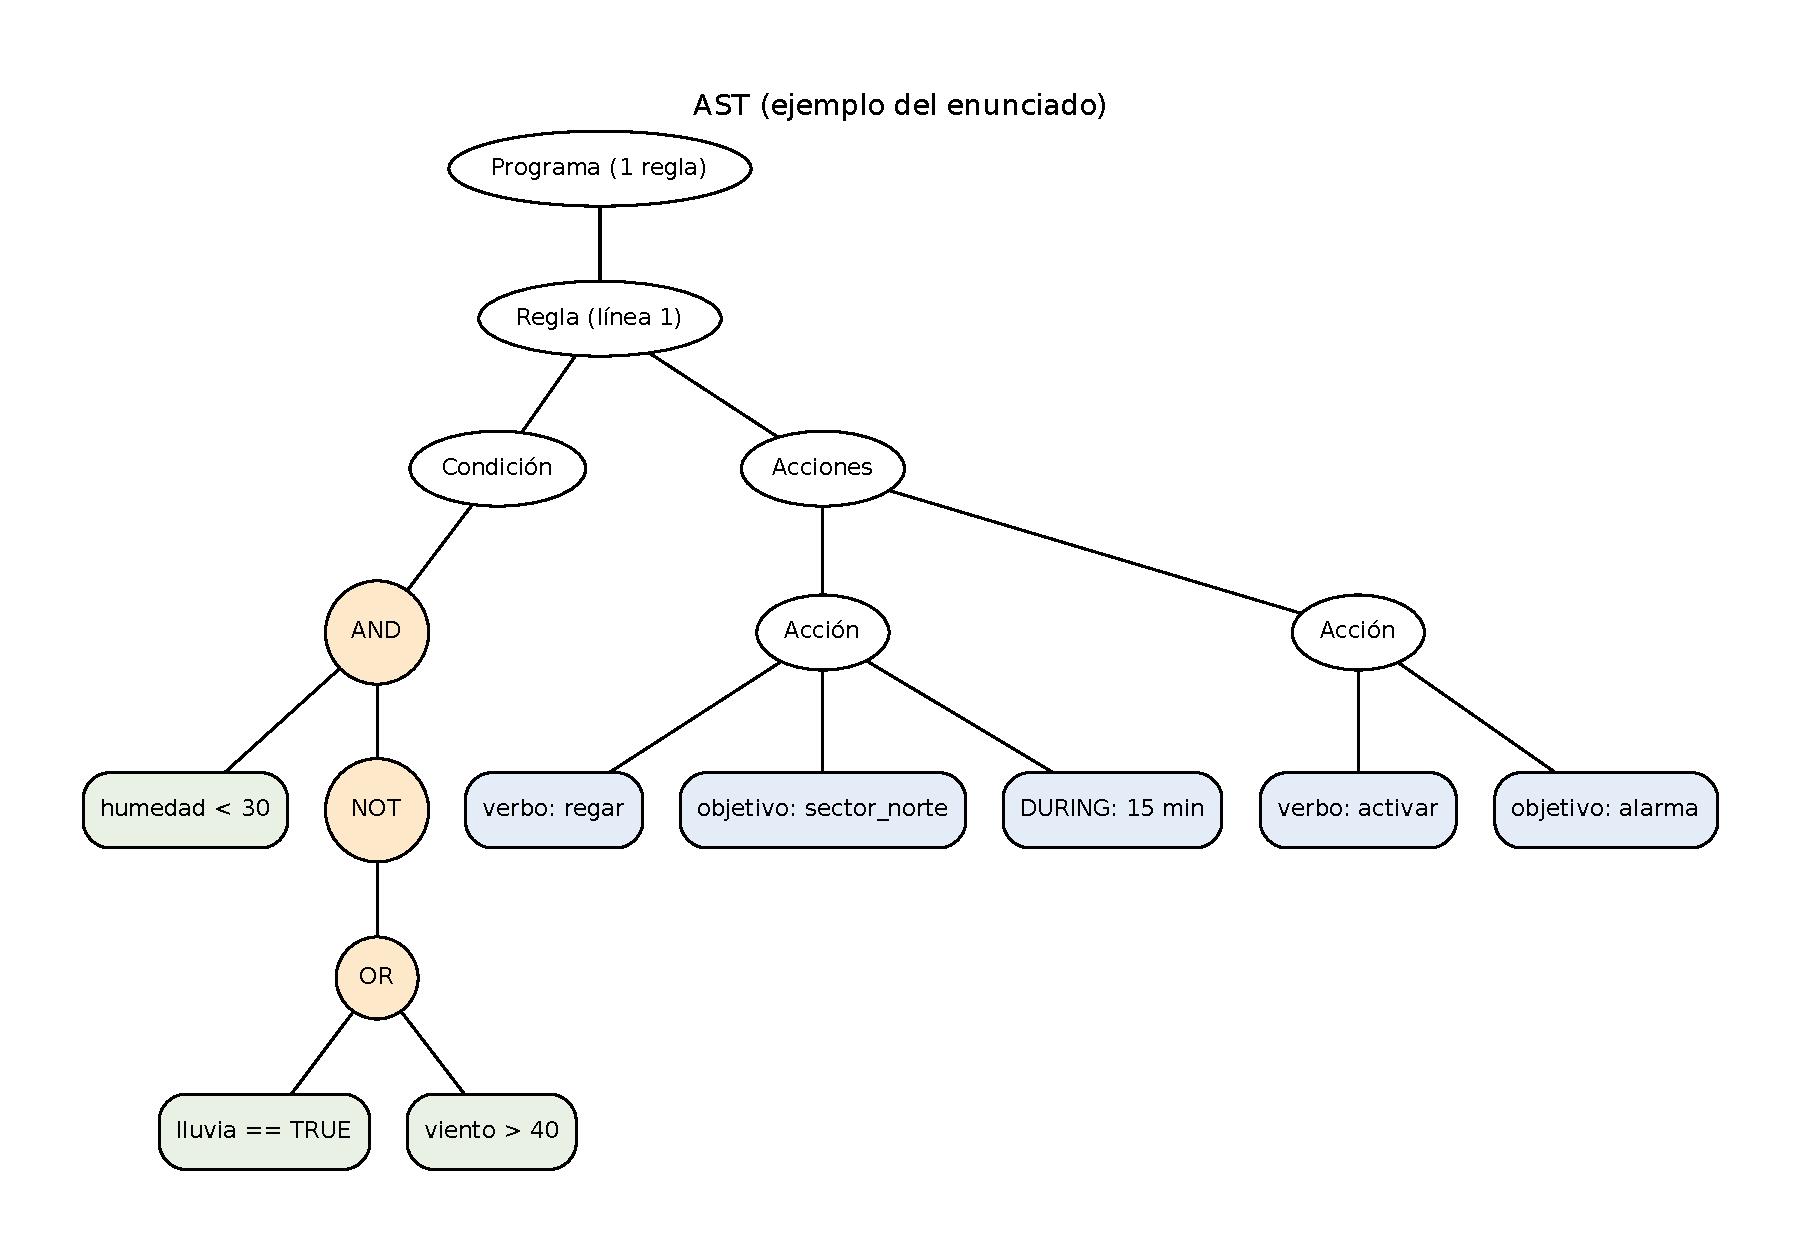
\includegraphics[width=0.9\linewidth]{../resultados/ast.pdf}
\caption{AST del ejemplo principal (Graphviz, generado con \T{--dot-ast}). Círculos: operadores lógicos; cajas verdes:
comparaciones; cajas azules: datos de cada acción, incluida la duración \T{DURING}.}\label{fig:ast}
\end{figure}

La misma estructura en texto (\T{python3 -m agroreglas ejemplos/riego.agro --ast --ascii} muestra también la segunda
regla del archivo):

\archivopeq{generado/ast.tex}

\subsection{Árbol concreto}
El árbol concreto de una regla corta muestra todos los símbolos de la derivación, incluidas las hojas \eps{} de las
producciones 3, 7, 10 y 20. Para \EntradaTraza{} (la misma entrada de la traza del anexo~\ref{sec:traza}):

\archivopeq{generado/arbol_concreto_traza.tex}

El árbol concreto del ejemplo principal tiene 65 nodos; su versión gráfica es la figura~\ref{fig:concreto} del
anexo y su versión en texto, \ruta{resultados/arbol_concreto.txt}. Para todas las entradas válidas de la batería, las
pruebas verifican dos propiedades del árbol concreto: (1) cada nodo interno aplica una producción de $G_2$ (sus hijos
son exactamente el lado derecho), y (2) la frontera ---las hojas leídas de izquierda a derecha, sin \eps--- es la
secuencia de tokens de la entrada.

% ====================================================================== 9
\section{Manejo de errores}\label{sec:errores}

\subsection{Estrategia}
El análisis se detiene en el primer error (no hay recuperación en modo pánico) y lo informa con toda la
información disponible. Hay dos clases de error, ambas subclases de \T{ValueError}:
\begin{itemize}
\item \textbf{\T{ErrorLexico}}: un carácter que no inicia ningún token. Incluye una sugerencia cuando el carácter es un
error típico (\T{=} por \T{==}, \T{!} por \T{!=}, coma, punto decimal, signo, comentario, comillas, letras no ASCII).
\item \textbf{\T{ErrorSintactico}}: la cima de la pila es un terminal distinto del token actual, la celda M[$A$, $a$]
está vacía o el token no es viable antes de una producción \eps.
\end{itemize}

\necesita{9\baselineskip}
\subsection{Contenido de un mensaje}
\begin{longtable}{>{\raggedright}p{3.8cm}p{12.0cm}}
\caption{Información incluida en cada error sintáctico.}\\
\hline\cabeza \textbf{Elemento} & \textbf{Descripción}\\\hline\endfirsthead
Ubicación & línea y columna (desde 1) y posición absoluta (desde 0) del token culpable. Si la entrada terminó antes de
tiempo, se señala justo después del último token, no después de los blancos finales.\\
Mensaje contextual & «se esperaba \textit{X} \textit{contexto}, pero se encontró \textit{Y}»; $X$ se redacta según el
punto de la gramática («un valor (número entero, TRUE o FALSE)», «el objetivo de la acción 'regar'», «la duración en
minutos») y el contexto según el token anterior («después del operador '<'»).\\
Encontrado & el token actual descrito por su categoría y lexema («la palabra reservada THEN», «el identificador
'basura'», «el fin de la entrada»).\\
Esperados & la lista exacta de categorías aceptables en ese punto, en el orden de las columnas de la tabla.\\
Cima de la pila & el símbolo que se estaba analizando; permite ubicar la fila de la tabla durante la defensa.\\
Línea y puntero & la línea del texto con \T{\textasciicircum} bajo el símbolo (solo en la consola).\\
Casos especiales & entrada vacía; contenido sobrante después de la última regla; \T{)} sin apertura; paréntesis
abierto sin cerrar (con su línea y columna); regla incompleta al final de la entrada.\\\hline
\end{longtable}

\subsection{Ejemplos reales}
Salidas de la consola tal como las imprime el programa (transcripciones de \ruta{resultados/transcripciones/}; las
líneas más largas se dividieron para caber en la página). Las capturas de pantalla de estas ejecuciones están en el
anexo~\ref{sec:evidencias}.

\archivopeq{generado/transcripcion_02_invalida_falta_valor.txt}
\archivopeq{generado/transcripcion_03_invalida_parentesis.txt}
\archivopeq{generado/transcripcion_04_invalida_truncada.txt}
\archivopeq{generado/transcripcion_06_invalida_sobrante.txt}
\archivopeq{generado/transcripcion_05_invalida_lexico.txt}

\subsection{Limitaciones del manejo de errores}
Se informa un solo error por ejecución. Una extensión natural sería la recuperación en modo pánico: descartar tokens
hasta \T{;} (que pertenece a FOLLOW(\NT{Acciones})) y reiniciar en \NT{Resto} para informar varios errores. Como el
léxico se ejecuta completo antes del parser, un error léxico tiene prioridad sobre un error sintáctico que aparezca
antes en el texto (lo documenta una prueba).

% ====================================================================== 10
\section{Casos de prueba}\label{sec:pruebas}

\subsection{Metodología}
Los casos están definidos en \ruta{tests/casos.py}. Para cada uno se fijó, antes de ejecutar el programa, el
veredicto esperado y, en los rechazos, el tipo de error (léxico o sintáctico), la línea y la columna del símbolo
culpable ---calculadas a mano--- y un fragmento que el mensaje debe contener. Un caso coincide solo si se cumplen
todos esos oráculos. Los resultados obtenidos de las tablas siguientes provienen de la ejecución del programa
(\ruta{resultados/pruebas.csv} y \cod{pruebas.json}); una prueba verifica que esos archivos coinciden con una nueva
ejecución. En los rechazos, «sint.» y «léxi.» indican el tipo de error y \textit{l}:\textit{c} su línea y columna.
Las entradas muy largas se muestran resumidas; el texto completo está en los archivos de resultados.

Resultado global: \textbf{\NumCorrectos{} de \NumCasos{} casos coinciden con lo esperado} (\NumValidas{} válidos,
\NumInvalidas{} inválidos y \NumLimite{} casos límite). La cantidad de casos no debe confundirse con la cantidad de
métodos de prueba: los \NumCasos{} casos se recorren dentro de un mismo método con subpruebas, y los \NumMetodos{}
métodos evalúan además otras entradas (sección~\ref{sec:adicionales}).

\setlength{\LTpre}{4pt}
\newcommand{\cabeceracasos}{\hline\cabeza \textbf{ID} & \textbf{Entrada} & \textbf{Esperado} & \textbf{Obtenido} & \textbf{Observación}\\\hline}

\necesita{9\baselineskip}
\subsection{Entradas válidas}
\begingroup\small\setlength{\tabcolsep}{4pt}
\begin{longtable}{p{0.75cm}>{\raggedright}p{6.0cm}>{\raggedright}p{2.35cm}>{\raggedright}p{2.6cm}>{\raggedright\arraybackslash}p{3.85cm}}
\caption{Entradas sintácticamente válidas (la línea gris resume el AST obtenido).}\\
\cabeceracasos\endfirsthead
\cabeceracasos\endhead
\filas{generado/casos_validos.tex}
\end{longtable}
\endgroup

\necesita{9\baselineskip}
\subsection{Entradas inválidas}
\begingroup\small\setlength{\tabcolsep}{4pt}
\begin{longtable}{p{0.75cm}>{\raggedright}p{6.0cm}>{\raggedright}p{2.35cm}>{\raggedright}p{2.6cm}>{\raggedright\arraybackslash}p{3.85cm}}
\caption{Entradas sintácticamente inválidas (la línea gris es el mensaje real del programa).}\\
\cabeceracasos\endfirsthead
\cabeceracasos\endhead
\filas{generado/casos_invalidos.tex}
\end{longtable}
\endgroup

\necesita{9\baselineskip}
\subsection{Casos límite}
Cubren la entrada vacía o solo con blancos, reglas truncadas, contenido sobrante, tokens sin espacios, ceros,
números y anidamientos muy grandes, 1000 reglas con CRLF, separadores inusuales, números con signo o decimales,
caracteres fuera del alfabeto, errores en una segunda línea y la frontera entre sintaxis y semántica.

\begingroup\small\setlength{\tabcolsep}{4pt}
\begin{longtable}{p{0.75cm}>{\raggedright}p{6.0cm}>{\raggedright}p{2.35cm}>{\raggedright}p{2.6cm}>{\raggedright\arraybackslash}p{3.85cm}}
\caption{Casos límite.}\\
\cabeceracasos\endfirsthead
\cabeceracasos\endhead
\filas{generado/casos_limite.tex}
\end{longtable}
\endgroup

\necesita{9\baselineskip}
\subsection{Comprobaciones adicionales}\label{sec:adicionales}
La batería \cod{unittest} tiene \NumMetodos{} métodos en siete módulos. La tabla~\ref{tab:adicionales} resume qué
comprueba cada grupo y cuántas entradas evalúa.

\begin{longtable}{>{\raggedright}p{3.4cm}>{\raggedright}p{9.0cm}>{\raggedright\arraybackslash}p{3.2cm}}
\caption{Comprobaciones automatizadas además de la tabla de casos.}\label{tab:adicionales}\\
\hline\cabeza \textbf{Aspecto} & \textbf{Qué se verifica} & \textbf{Entradas}\\\hline\endfirsthead
\hline\cabeza \textbf{Aspecto} & \textbf{Qué se verifica} & \textbf{Entradas}\\\hline\endhead
Compatibilidad con el lexer docente (\ruta{test_lexico}) & igualdad de pares o de \T{ValueError} con la función
original ejecutada desde el notebook; salida registrada por el docente; diferencias M1, M4 y M5; MD5 del notebook
preservado & 42 casos, \NumComparadasLexico{} cadenas aleatorias\\
Posiciones y errores léxicos & línea, columna y posición de cada token y de \T{EOF}; CRLF; mayúsculas; coincidencia más
larga; ubicación y sugerencia de 8 errores léxicos & 17 entradas\\
FIRST/FOLLOW y tabla (\ruta{test_gramatica}) & $N$, $T$, $S$, $P$; anulables; FIRST, FOLLOW y SELECT de todo contra el
cálculo manual; las 31 celdas y las 179 de error; decisiones de \T{DURING}, \T{AND} y precedencia; G0 y G1 con sus
conflictos; recursión indirecta y conflicto en gramáticas de libro & 5 gramáticas\\
Consumo completo (\ruta{test_parser}) & 8 tipos de contenido sobrante, 5 reglas truncadas, frontera $=$ entrada &
13 + 25 aceptadas\\
Tokens del lexer docente & el parser acepta los pares \T{(TIPO, lexema)} y da el mismo veredicto que con texto;
secuencias mal formadas & 38 casos\\
Detección inmediata & mismo veredicto y posición con y sin la comprobación de viables; esperados exactos &
\NumCasos{} + \NumMutacionesInmediata{} entradas\\
Prueba diferencial & parser LL(1) frente a un reconocedor de Earley sobre G0, G1 y G2; oraciones aleatorias de G0 &
\NumDiferenciales{} + \NumOracionesGcero{} secuencias\\
Árbol y AST (\ruta{test_arboles}) & producciones del árbol concreto, frontera, derivación por la izquierda, precedencia,
agrupación, asociatividad, \T{DURING}, varias reglas y acciones, valores y lexemas, entradas grandes, Graphviz &
25 aceptadas + 24 específicas\\
Mensajes (\ruta{test_errores}) & ubicación, encontrado, esperados en 11 puntos de la gramática, puntero con
tabulaciones, 9 mensajes contextuales, primer error, prioridad del léxico & 25 entradas\\
Consola (\ruta{test_cli}) & códigos 0, 1 y 2 con los \NumEjemplos{} archivos de ejemplo, texto, stdin, BOM, UTF-8 inválido,
opciones de salida y exportación & \NumEjemplos{} archivos y 12 comandos\\
Coherencia (\ruta{test_resultados}) & \cod{analisis.json} y \cod{pruebas.json} coinciden con una nueva ejecución &
\NumCasos{} casos\\\hline
\end{longtable}

En la prueba diferencial, de las \NumDiferenciales{} secuencias el parser aceptó \NumDiferencialesAceptadas{} y
rechazó \NumDiferencialesRechazadas{}, exactamente las mismas que el reconocedor de Earley sobre G0. El reconocedor de
Earley (\ruta{tests/oraculos.py}) es un algoritmo general que no usa FIRST, FOLLOW ni la tabla, por lo que sirve como
oráculo independiente; se usa solo en las pruebas, no en el producto. La salida completa de la ejecución de las pruebas
está en el anexo~\ref{sec:unittest}.

% ====================================================================== 11
\section{Conclusiones y limitaciones}\label{sec:conclusiones}

\begin{itemize}
\item Se definió AgroReglas, un DSL para reglas de riego con 8 palabras reservadas, identificadores, valores enteros y
booleanos, seis operadores relacionales, tres lógicos con precedencia \T{NOT} $>$ \T{AND} $>$ \T{OR}, agrupación,
varias reglas, varias acciones y la extensión de dominio \T{DURING}.
\item La gramática se obtuvo en tres pasos medidos con el mismo programa: G0 (ambigua, recursiva por la izquierda y
con prefijos comunes; \NumConflictosGcero{} conflictos), G1 (precedencia; \NumConflictosGuno{} conflictos) y G2 (sin
recursión ni prefijos; 0 conflictos). G2 es LL(1) y, por lo tanto, no ambigua; una prueba diferencial con Earley
respalda que las tres generan el mismo lenguaje.
\item FIRST, FOLLOW, los conjuntos de selección y la tabla se calculan con algoritmos propios de punto fijo y
coinciden con el cálculo manual. Una sola definición de la gramática alimenta el análisis, el parser, los
resultados y las tablas de este informe.
\item El parser predictivo dirigido por tabla acepta y rechaza según los oráculos en los \NumCasos{} casos, consume
toda la entrada, construye el árbol concreto y el AST y entrega errores con línea, columna, símbolo encontrado y
símbolos esperados exactos.
\end{itemize}

\textbf{Limitaciones.}
\begin{itemize}
\item Solo reconocimiento: no hay intérprete ni control de equipos, y no se validan tipos, unidades, rangos ni la
existencia de sensores y equipos (L21 se acepta).
\item Se informa un único error por ejecución (sin recuperación) y el léxico completo precede al parser.
\item El lenguaje no admite decimales, negativos, comentarios, comparaciones entre sensores ni estructuras como
\T{IF--ELSE} o bloques; las reservadas no distinguen mayúsculas, decisión heredada de la función docente.
\item Las pruebas aleatorias y diferenciales aumentan la confianza, pero no reemplazan el argumento formal: muestran
que no se encontraron discrepancias en las entradas evaluadas.
\end{itemize}
Como trabajo futuro se propone una fase semántica separada (catálogo de sensores y acciones, tipos de valores, duración
positiva), recuperación de errores en \T{;} y comentarios de línea.

% ====================================================================== 12
\clearpage
\section{Anexos}\label{sec:anexos}

\subsection{Anexo A. Repositorio, contenido de la entrega y reproducción}\label{sec:repositorio}
Código fuente, README, ejemplos, pruebas, resultados, notebook, informe y archivos auxiliares:
\begin{center}\url{https://github.com/der-kaffe/AgroReglas-LL1}\end{center}
Estructura de la entrega:

\begin{codigo}
\begin{verbatim}
Proyecto_AgroReglas/
  README.md               instrucciones, dependencias, formato de entrada y ejemplos
  agroreglas/             código fuente: lexico, gramatica, ll1, parser, arbol,
                          abstracto, errores y la interfaz de consola
  tests/                  casos con oráculos, oráculos independientes y 7 módulos
  ejemplos/               riego.agro, error.agro, validos/ e invalidos/
  generar_resultados.py   regenera resultados/ y documentacion/generado/
  herramientas/           capturas de terminal (Xvfb) y ejecución del notebook
  resultados/             gramatica.txt, analisis.json, first_follow.csv,
                          seleccion.csv, tabla_ll1.csv/.md, pruebas.csv/.json,
                          árboles (.txt/.dot/.png/.pdf), derivacion.txt, traza.txt,
                          transcripciones/ y capturas/
  documentacion/          Informe_AgroReglas.pdf/.tex, generado/, AgroReglas.ipynb
                          (ejecutado) y anlizador_lexico1.ipynb (original del
                          docente)
\end{verbatim}
\end{codigo}

Reproducción desde una copia limpia: \T{python3 -m unittest discover -s tests -v}, luego
\T{python3 generar\_resultados.py} y, para el informe, \T{pdflatex Informe\_AgroReglas.tex} tres veces dentro de
\ruta{documentacion/}. El informe usa solo paquetes básicos de LaTeX (\cod{babel}, \cod{geometry}, \cod{longtable},
\cod{colortbl}, \cod{graphicx}, \cod{hyperref}, \cod{fancyhdr}, \cod{verbatim}, \cod{amssymb}).

\necesita{9\baselineskip}
\subsection{Anexo B. Trazabilidad con la rúbrica}
La tabla relaciona cada criterio con la evidencia entregada. Describe lo que contiene la entrega; no asigna ni
garantiza una calificación.

\begin{longtable}{>{\raggedright}p{3.6cm}>{\raggedright}p{6.4cm}>{\raggedright\arraybackslash}p{5.6cm}}
\caption{Trazabilidad entre criterios de la rúbrica y evidencias.}\\
\hline\cabeza \textbf{Criterio (puntos)} & \textbf{Evidencia en el informe} & \textbf{Evidencia en archivos}\\\hline\endfirsthead
\hline\cabeza \textbf{Criterio (puntos)} & \textbf{Evidencia en el informe} & \textbf{Evidencia en archivos}\\\hline\endhead
1. Lenguaje y dominio (10) & Secc. 1--2: dominio, alfabeto, tokens, reservadas, restricciones, 6 + 6 ejemplos explicados,
lexer y compatibilidad & \cod{lexico.py}, \ruta{ejemplos/}, \ruta{test_lexico.py}\\
2. GLC (15) & Secc. 3: $G=(N,T,P,S)$ completa, convenciones $\varepsilon$/\T{EOF}, derivación por la izquierda &
\cod{gramatica.py}, \ruta{resultados/gramatica.txt}, \cod{derivacion.txt}\\
3. Análisis, FIRST y FOLLOW (20) & Secc. 4--5: G0/G1/G2, ambigüedad, recursión directa e indirecta, factorización,
precedencia, FIRST/FOLLOW justificados & \cod{ll1.py}, \cod{analisis.json}, \ruta{first_follow.csv},
\ruta{test_gramatica.py}\\
4. Tabla LL(1) (10) & Secc. 6: SELECT, disjunción, matriz completa, conflictos de G0 y G1 & \ruta{tabla_ll1.csv/.md},
\cod{seleccion.csv}\\
5. Parser (20) & Secc. 7: arquitectura, algoritmo, código real, producciones y código, complejidad, CLI &
\cod{parser.py}, \ruta{test_parser.py}, \ruta{test_cli.py}, anexos C--E\\
6. Árbol/AST y errores (10) & Secc. 8--9: árbol concreto y AST diferenciados, figuras, mensajes y ejemplos reales &
\cod{arbol.py}, \cod{abstracto.py}, \cod{errores.py}, \ruta{test_arboles.py}, \ruta{test_errores.py}\\
7. Pruebas y extensión (10) & Secc. 4.8 y 10: \NumCasos{} casos con resultado obtenido, comprobaciones adicionales,
\T{DURING} integrada & \ruta{tests/}, \ruta{pruebas.csv/.json}, \ruta{transcripciones/}\\
8. Informe y README (5) & Este informe y sus anexos & \cod{README.md}, notebook ejecutado y
fuente LaTeX\\
Criterios transversales & Solución ejecutable; desarrollo propio sin generador; correspondencia informe--código por
generación automática; extensión integrada & \ruta{generar_resultados.py}, \ruta{test_resultados.py}\\\hline
\end{longtable}

\necesita{9\baselineskip}
\subsection{Anexo C. Evidencias de ejecución}\label{sec:evidencias}
Las figuras~\ref{fig:cap1} a \ref{fig:cap6} son \textbf{capturas de pantalla reales de una terminal xterm} que ejecuta
los comandos indicados en el directorio del proyecto. Se obtuvieron con \ruta{herramientas/capturar_terminal.sh}, que
abre la terminal en un servidor gráfico virtual (Xvfb) y la captura con ImageMagick; por eso no muestran la barra de
título de un escritorio. Cada comando aparece precedido de \T{\$} y seguido de su código de salida real. Las mismas
ejecuciones están como texto en \ruta{resultados/transcripciones/}.

\begin{figure}[htbp]\centering
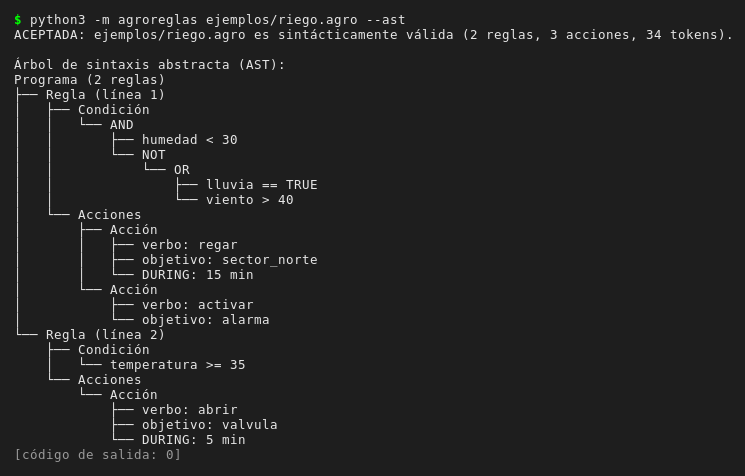
\includegraphics[width=0.78\linewidth]{../resultados/capturas/01_entrada_valida.png}
\caption{Entrada válida: dos reglas reconocidas y su AST (código de salida 0).}\label{fig:cap1}
\end{figure}

\begin{figure}[htbp]\centering
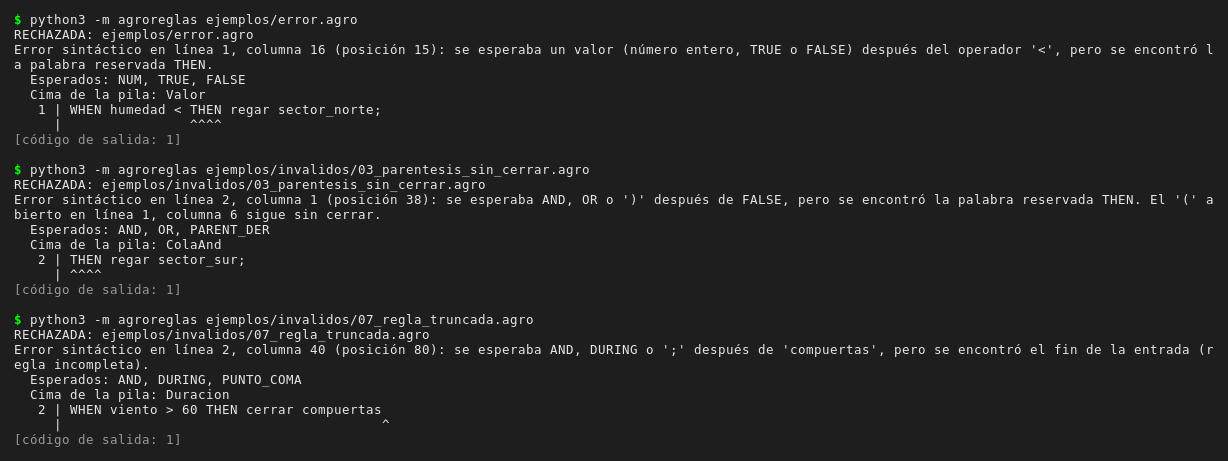
\includegraphics[width=\linewidth]{../resultados/capturas/02_errores_sintacticos.png}
\caption{Errores sintácticos: valor faltante, paréntesis sin cerrar y regla truncada (código 1).}\label{fig:cap2}
\end{figure}

\begin{figure}[htbp]\centering
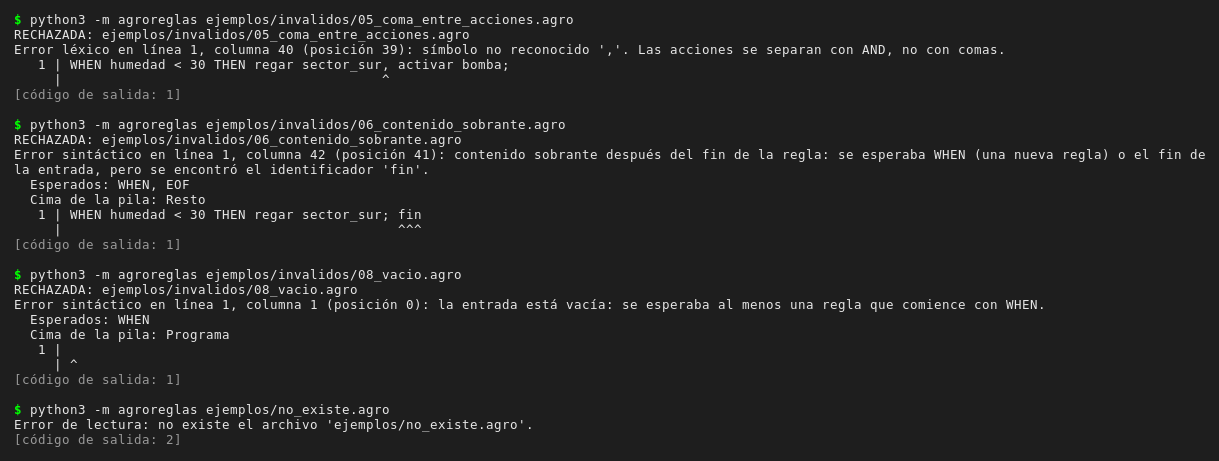
\includegraphics[width=\linewidth]{../resultados/capturas/03_lexico_limites_y_uso.png}
\caption{Error léxico, contenido sobrante, entrada vacía (código 1) y archivo inexistente (código 2).}\label{fig:cap3}
\end{figure}

\begin{figure}[htbp]\centering
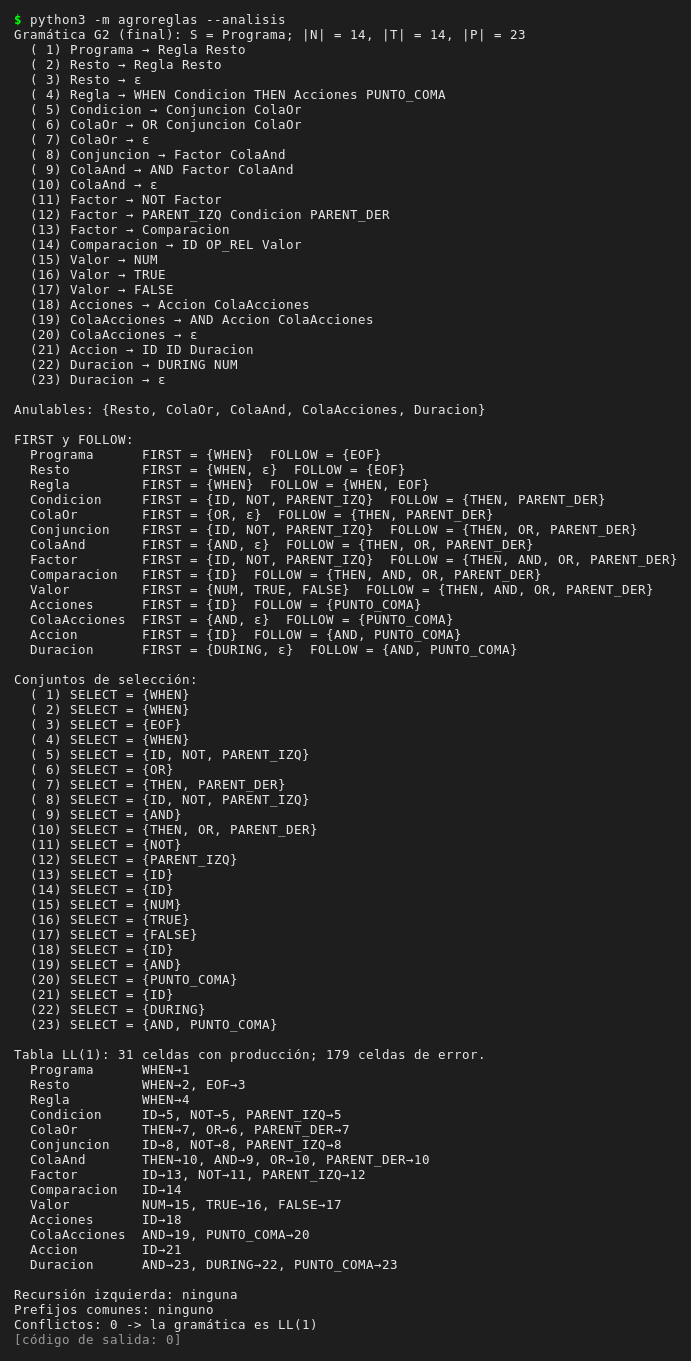
\includegraphics[height=0.86\textheight]{../resultados/capturas/04_analisis_gramatica.png}
\caption{\T{--analisis}: gramática, anulables, FIRST, FOLLOW, SELECT, tabla LL(1) y ausencia de conflictos.}\label{fig:cap4}
\end{figure}

\begin{figure}[htbp]\centering
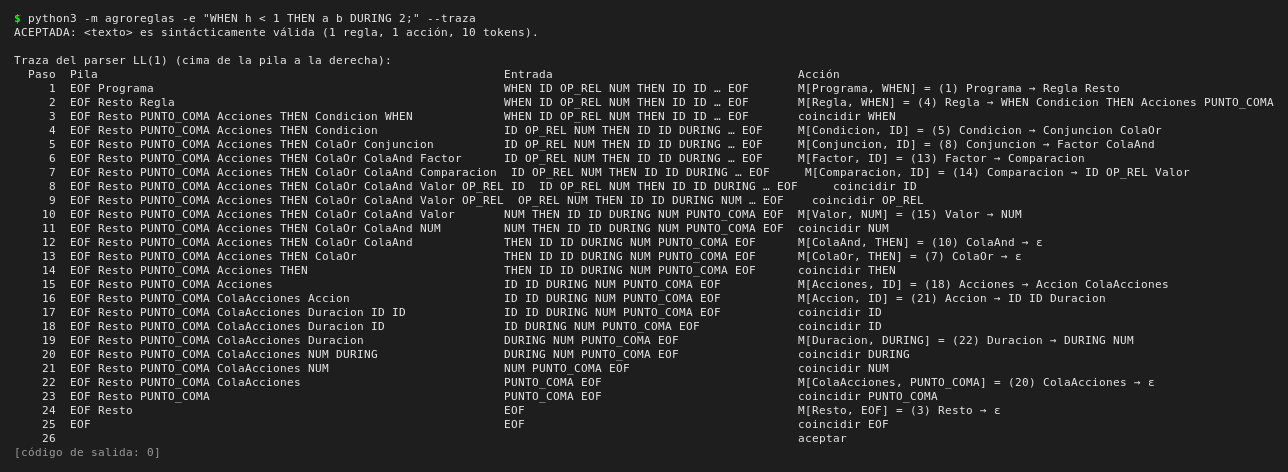
\includegraphics[width=\linewidth]{../resultados/capturas/05_traza_ll1.png}
\caption{Traza del parser LL(1) para \T{WHEN h < 1 THEN a b DURING 2;}: pila, entrada y acción en cada paso.}\label{fig:cap5}
\end{figure}

\begin{figure}[htbp]\centering
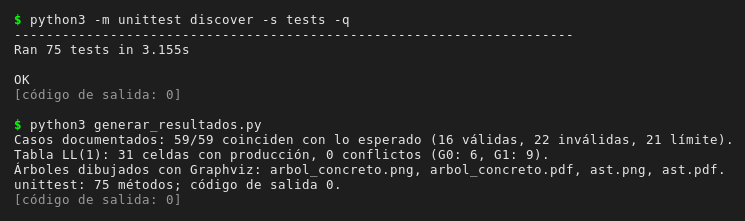
\includegraphics[width=0.78\linewidth]{../resultados/capturas/06_pruebas_y_resultados.png}
\caption{Ejecución de la batería \cod{unittest} y regeneración de resultados.}\label{fig:cap6}
\end{figure}

\begin{figure}[htbp]\centering
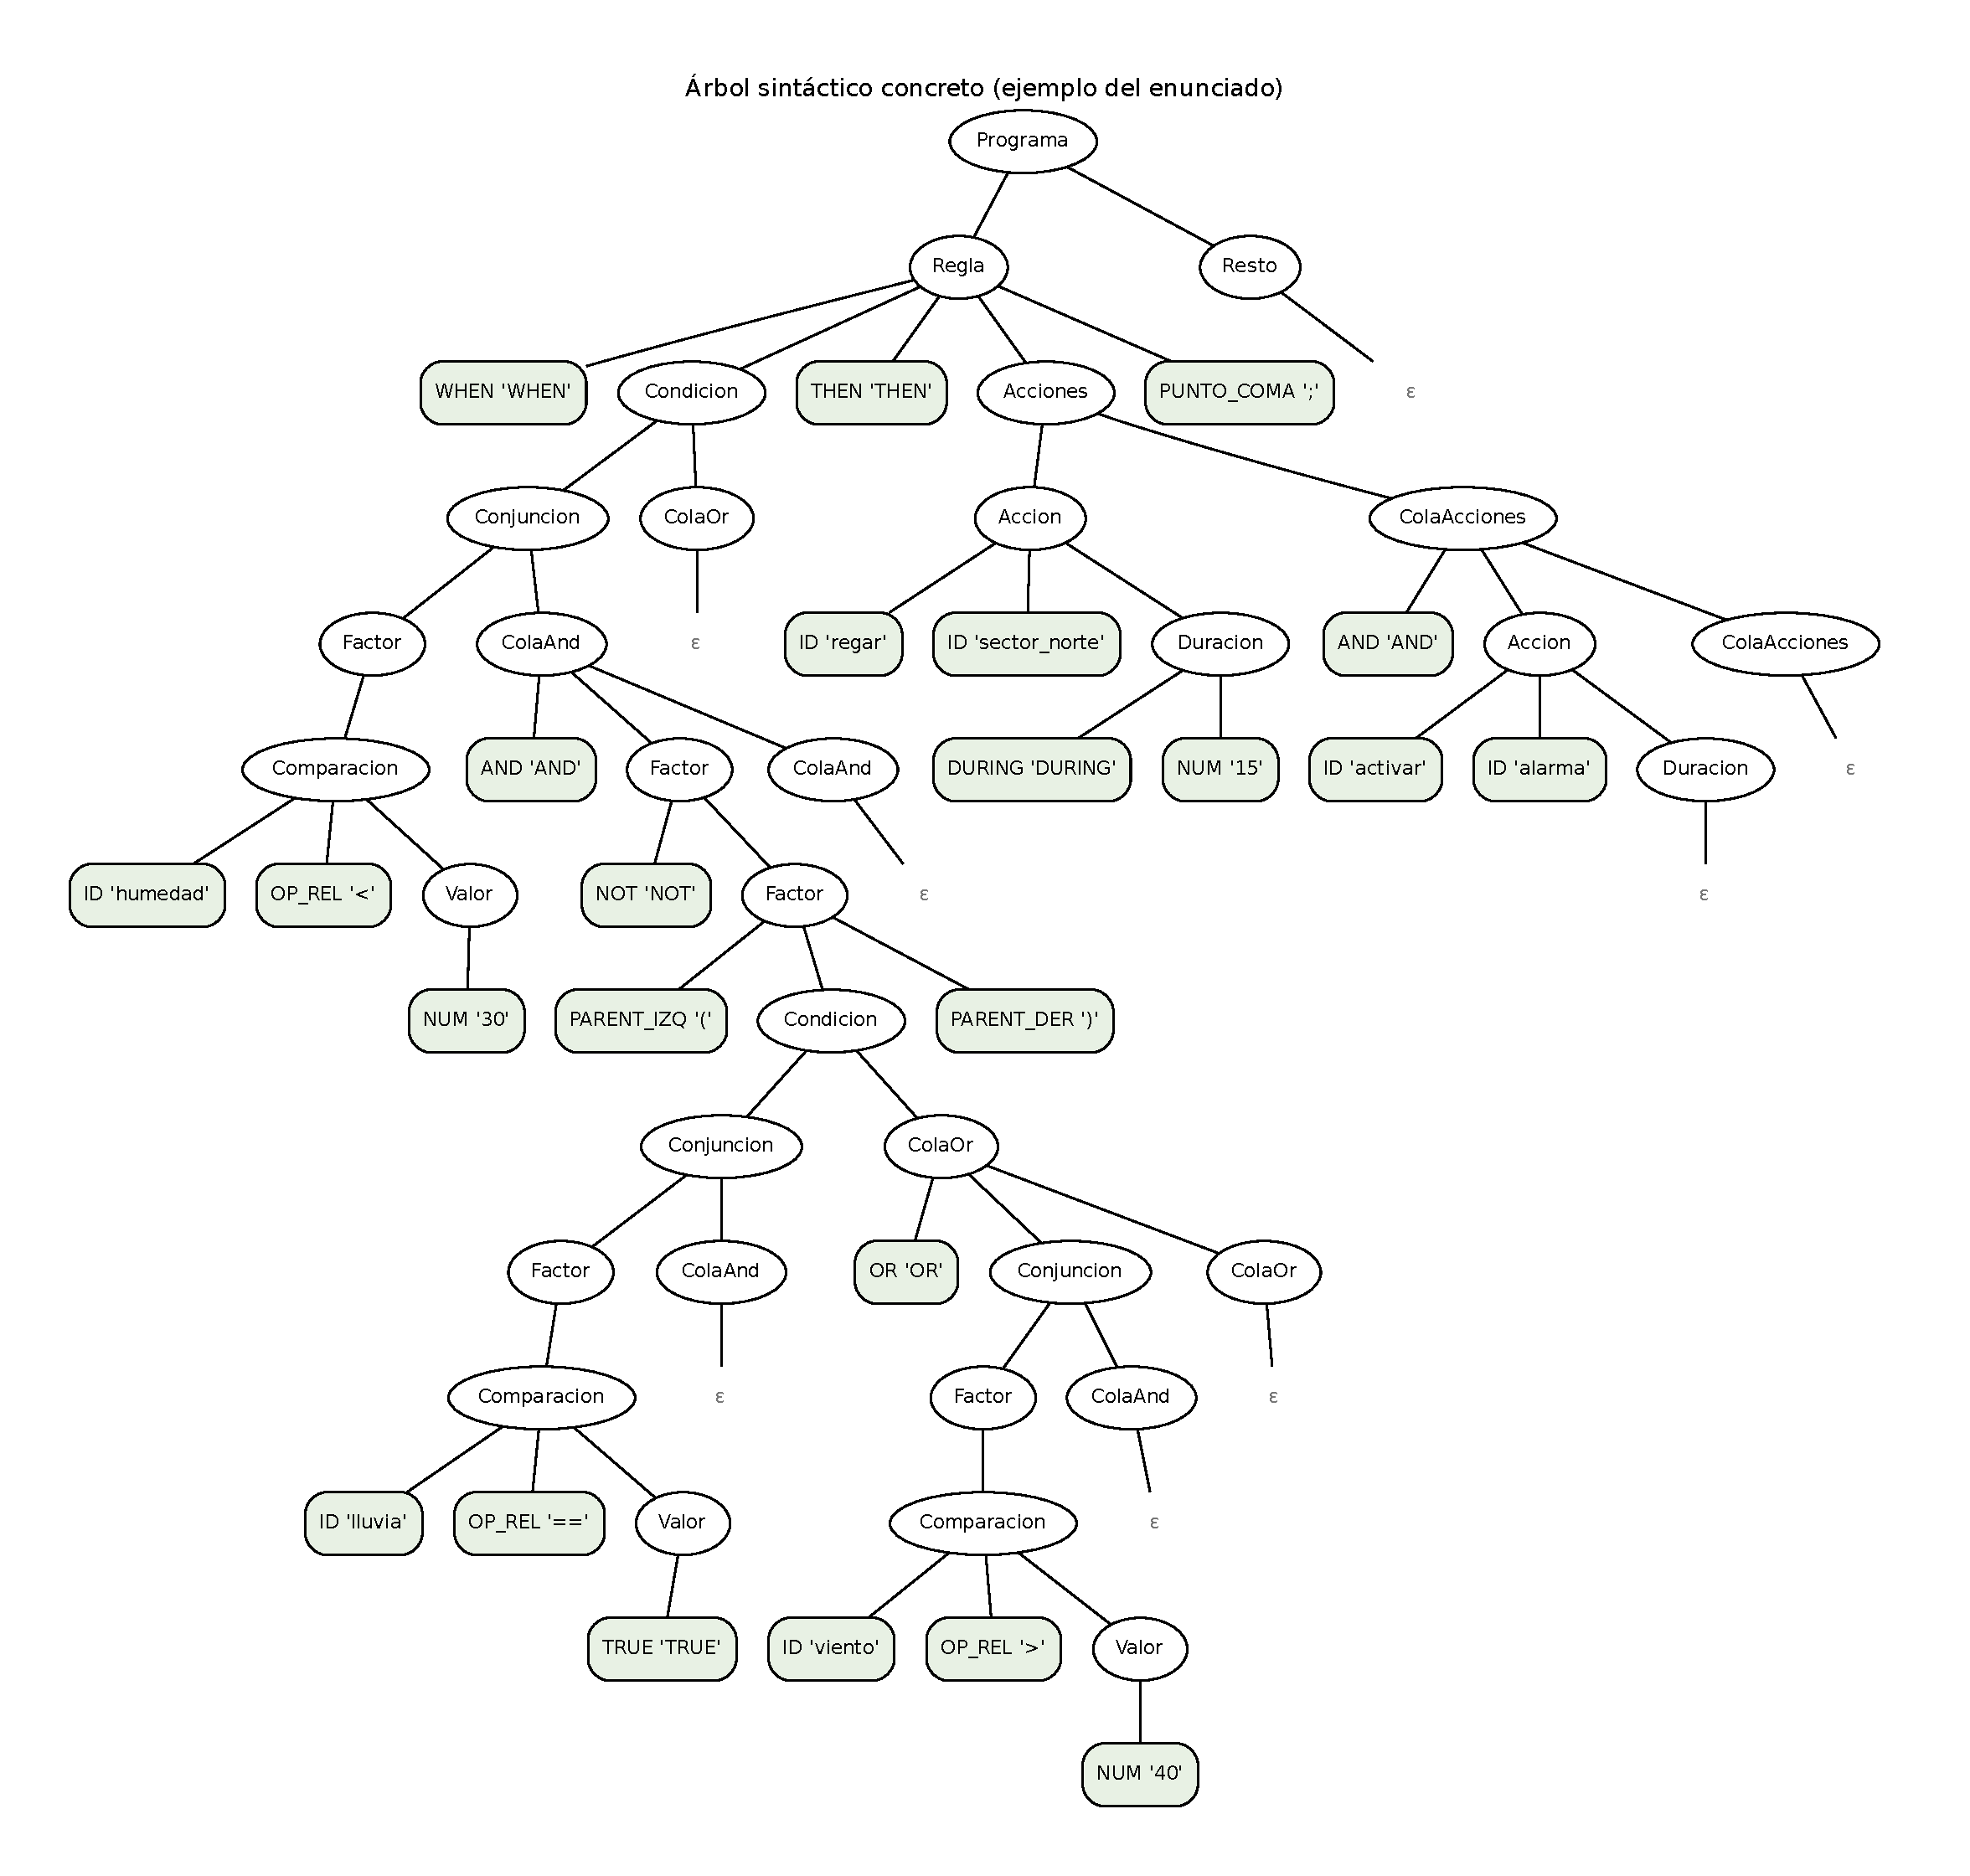
\includegraphics[width=\linewidth,height=0.8\textheight,keepaspectratio]{../resultados/arbol_concreto.pdf}
\caption{Árbol sintáctico concreto del ejemplo principal (Graphviz; figura vectorial, se puede ampliar en el PDF).
Elipses: no terminales; cajas: tokens; texto gris: \eps.}\label{fig:concreto}
\end{figure}

\clearpage
Resultado de ejecutar la consola sobre cada archivo de \ruta{ejemplos/} (transcripción real):

\archivomin{generado/transcripcion_00_todos_los_ejemplos.txt}

\necesita{9\baselineskip}
\subsection{Anexo D. Traza completa del parser LL(1)}\label{sec:traza}
Traza para \EntradaTraza{} (\PasosTraza{} pasos). La pila se escribe con la cima a la derecha; «coincidir» indica que la
cima era el terminal actual y se consumió.

\begingroup\footnotesize\setlength{\tabcolsep}{3.5pt}
\begin{longtable}{r>{\raggedright}p{5.6cm}>{\raggedright}p{4.0cm}>{\raggedright\arraybackslash}p{5.6cm}}
\hline\cabeza \textbf{Paso} & \textbf{Pila} & \textbf{Entrada} & \textbf{Acción}\\\hline\endfirsthead
\hline\cabeza \textbf{Paso} & \textbf{Pila} & \textbf{Entrada} & \textbf{Acción}\\\hline\endhead
\filas{generado/traza.tex}
\hline
\end{longtable}
\endgroup

\necesita{9\baselineskip}
\subsection{Anexo E. Ejecución de la batería de pruebas}\label{sec:unittest}
Salida completa y real de \T{python3 -m unittest discover -s tests -v} (las líneas largas se dividieron):

\archivomin{generado/transcripcion_11_unittest.txt}

\end{document}
